%!TEX encoding = UTF-8 Unicode
\documentclass[
	a4paper,
	twoside,
	justified
]{tufte-book}
\usepackage{../common/common}
\usetikzlibrary{automata}
%\usepackage{subfiles}
\usepackage{siunitx}
%\usepackage[options]{natbib}
\renewcommand{\rmdefault}{pplx}\usetikzlibrary{plotmarks}
\usetikzlibrary{arrows.meta}
\usetikzlibrary{decorations.pathreplacing}
\graphicspath{{./img/}}

\bibliographystyle{alpha}

\setcounter{secnumdepth}{1}

\title{Patrons de Connexió \\
				al CV de la UOC}
\date{gener del 2015}
\author{Armand Adroher Salvia\\
	{\it UOC - TFG - EDM\&LA}}
 
\begin{document}

\setcounter{tocdepth}{1}
  
\frontmatter\pagenumbering{roman}

\maketitle

\newpage
\begin{fullwidth}
~\vfill
\thispagestyle{empty}
\setlength{\parindent}{0pt}
\setlength{\parskip}{\baselineskip}

\par Aquesta és la memòria lliurada en motiu de la realització del \emph{Treball de Fi de Grau} en el marc del programa \emph{Educational Data Mining and Learning Analytics} durant el transcurs del semestre de tardor del curs 2014-2015.  

\index{license}

\end{fullwidth}


\tableofcontents

\listoffigures

\listoftables

\cleardoublepage
\chapter*{Resum}

La disciplina de la \emph{Educational Data Ming and Learning Analytics} té per objecte emprar els mètodes propis de la \emph{Descoberta de Coneixement en Bases de Dades} i l'\emph{Aprenentatge Computacional} amb la finalitat de comprendre i millorar, si s'escau, els processos que tenen lloc en entorns d'aprenentatge. En aquest estudi es parteix d'un registre d'establiment i clausura de sessions dels usuaris al \emph{Campus Virtual} de la \emph{UOC} per a mirar d'obtenir resultats en aquesta direcció. Amb la finalitat d'ésser fidels a la informació que proporcionen les dades, en proposo una discretització que mesura la presència o absència, al \emph{Campus Virtual}, de cada un dels usuaris, en funció de determinats intervals temporals. Això m'ha permès aplicar mètodes d'agregació que han donat lloc a un esbós de tipologia de comportament d'usuaris en el transcurs del semestre. En darrer lloc, el resultat central d'aquest estudi és l'obtenció d'un mètode simple per a l'estimació de models ocults de Markov que siguin capaços de predir, per a cada moment del desplegament temporal del semestre i amb un alt grau d'encerts, el trencament de la relació amb el \emph{Campus Virtual} per part de cada usuari.           


\mainmatter\setcounter{page}{1}\pagenumbering{arabic}

\chapter{Determinació d'objectius}

Encetem aquest estudi tot establint-ne el punt de partida i enunciant l'objectiu genèric d'anàlisi de dades que l'ha motivat.

\section{Motivació de l'estudi}

En motiu de la realització d'aquest treball de fi de grau (TFG), la UOC em va fer arribar un fitxer de text pla\footnote{El fitxer en qüestió acompanya el lliurament d'aquesta memòria amb el nom \texttt{20131.con.txt} .} que consistia en la representació d'una taula mitjançant el format \emph{Comma Separated Values} (CSV). Presenta una estructura molt simple, en cada una de les línies de text que el componen hi trobem 4 valors. A partir de la informació que va acompanyat-ne el lliurament podem afirmar que:
 
\begin{enumerate}[(1)]
  \item Aquestes dades són extretes dels registres de sessions establertes al programari web que implementa el Campus Virtual de la UOC (CV).
  \item Els 4 camps a què corresponen cada un dels valors respectius són:
  \begin{enumerate}[(a)]
    \item Una seqüència de dígits decimals, que és un identificador de l'usuari que ha establert aquesta sessió.
    \item Les 3 marques de temps (\emph{timestamp}) següents\footnote[][-3\baselineskip]{Si emprem la notació que admet la funció \texttt{strftime}, totes les marques de temps del fitxer segueixen el format ``\texttt{\%d/\%m/\%Y \%H:\%M:\%S}'', és a dir, tenen una precisió d'1 segon}:
    \begin{enumerate}[(i)] 
 		\item La primera indica el moment en què s'ha iniciat la sessió al CV en nom d'aquest usuari.
    \item La segona indica el moment en què s'ha realitzat la darrera petició al CV de la UOC dins d'aquesta sessió.
    \item La darrera consisteix en el moment en què ha caducat la sessió.
    \end{enumerate}  
  \end{enumerate}  
\end{enumerate}

A mode d'exemple, la figura \ref{20131.con.txt_head} es mostra les primeres quatre línes d'aquest fitxer. 

\begin{figure*}
\usemintedstyle{trac}
\begin{minted}[linenos=true,
                bgcolor=mintedbg,
                fontfamily=tt,
                %numbersep=-2\tabcolsep,
                numbersep=.5pt,
                gobble=0,
                fontsize=\small,
                frame=lines,
                framesep=\baselineskip,
                xleftmargin=2\tabcolsep,
                baselinestretch=0.75,
                tabsize=2
								]{text}
7149084242663;18/09/2013 00:00:03;18/09/2013 00:57:28;18/09/2013 02:04:32
6059394219413;18/09/2013 00:00:04;18/09/2013 00:00:15;18/09/2013 01:07:21
4139154106177;18/09/2013 00:00:07;18/09/2013 00:31:29;18/09/2013 01:39:07
858883854230;18/09/2013 00:00:07;18/09/2013 00:00:12;18/09/2013 01:07:21
\end{minted}
\caption{
	\label{20131.con.txt_head}
	Primeres quatre línies del fitxer \texttt{20131.con.txt}
}
\end{figure*}

El programa en què s'emmarca aquest TFG proposava com a objectiu general aplicar, a aquest conjunt de dades les tècniques pròpies les disciplines d'\emph{Educational Data Mining} i \emph{Learning Analytics} (EDM\&LA). En concordança llur naturalesa, aquest objectiu genèric es podria fer explícit, doncs, de la manera següent:

\begin{shaded}
  Emprar les tècniques pròpies del \emph{Descobriment de Coneixement en Bases de Dades} (KDD) i de l'\emph{Aprenentatge Computacional} (ML) en aquest conjunt de dades amb la finalitat d'obtenir coneixement que millori els processos que tenen lloc en entorns d'aprenentatge (en aquest cas, el CV de la UOC).      
\end{shaded}

En quins objectius concrets ha acabat reduint-se aquesta directiva general ha estat condicionat per part dels dos factors següents:

\begin{enumerate}[(1)]
\item Les característiques de les dades mateixes.
\item El grau de coneixement que he pogut obtenir sobre el procés que les ha produïdes. 
\end{enumerate}

\section{Naturalesa de les dades rebudes}
\label{sec:natu_dades_rebudes}

Proporciono, a continuació, un esbós de quina és la primera abstracció que realitzarem a partir d'aquestes dades, així com també un resum de quina és la dimensió del conjunt que en resulta. 

\subsection{Abstracció elemental}

Amb la finalitat de facilitar la notació en l'exposició, convenim que anomenarem \texttt{session} la classe dels objectes representats per part de cada una de les entrades del fitxer \mt{20131.con.txt}, i \mt{sessions} la relació que en resulta. Per altra banda, denotarem de la manera següent els atributs de l'esquema que la compon\footnote[][-2\baselineskip]{Noti's que s'hi ha afegit un atribut, \texttt{id}, amb un identificador únic per a assegurar-nos que es compleix el model relacional.}:

$$
\texttt{session(id, user\_id, session\_start, last\_request, session\_expiration)}
$$

Interpretarem que les seqüències de caràcters que integren les dades rebudes representen valors que pertanyen als tipus següents:

\begin{enumerate}[(1)]
	\item \texttt{id} $\in \mathbb{N}$
	\item \texttt{user\_id} $\in ([\mt{``0''},\mt{``9''}] \cup \mt{`` ''})^{13}$
	\item \texttt{session\_start} $\in$ \mt{timestamp}
	\item \texttt{last\_request} $\in$ \mt{timestamp}
	\item \texttt{session\_expiration} $\in$ \mt{timestamp}
\end{enumerate}

On $([$\mt{``0''}$,$\mt{``9''}$]\cup \mt{`` ''})^{13}$ són les seqüenciès de longitud 13 construïbles mitjançant els dígits numèrics i l'espai, i \mt{timestamp} és la marca de temps amb precisió de segons a què m'he referit anteriorment. Per altra banda, també definirem els següents atributs derivats:

\begin{fullwidth}
\begin{enumerate}[(1)]
	\setcounter{enumi}{5}
	\vspace{2\parskip}
	\item $\texttt{total\_duration} := [\texttt{session\_expiration}, \texttt{session\_start}) \in \texttt{interval}$
	\item $\texttt{activity\_duration} := [\texttt{last\_request}, \texttt{session\_start}) \in \texttt{interval}$
	\item $\texttt{inactivity\_duration} := [\texttt{session\_expiration}, \texttt{last\_request}) \in \texttt{interval}$
	\item $\texttt{central\_activity\_point} :=
	 (\texttt{session\_start} + \texttt{activity\_duration}) / 2 \in \texttt{timestamp}$ 
		\vspace{2\parskip}
\end{enumerate}
\end{fullwidth}

On \mt{iterval} representa un interval tancat de valors consecutius del tipus \mt{timestamp}. 

En darrer lloc, també utilitzarem la funció $l$ definida de la manera següent\footnote{És a dir, la llargada, en segons, d'un valor del tipus \texttt{interval}}:

\begin{align*}
l : \texttt{interval} & \rightarrow (\mathbb{N} \times \SI{}{\second}) \\
[t_0, t_1] & \mapsto t_1 - t_0   
\end{align*}

Podem dir que cada sessió es compon, doncs, de dos segments temporals consecutius. En la figura \ref{dia:session_structure} se'n mostra una representació gràfica.

\begin{figure*}
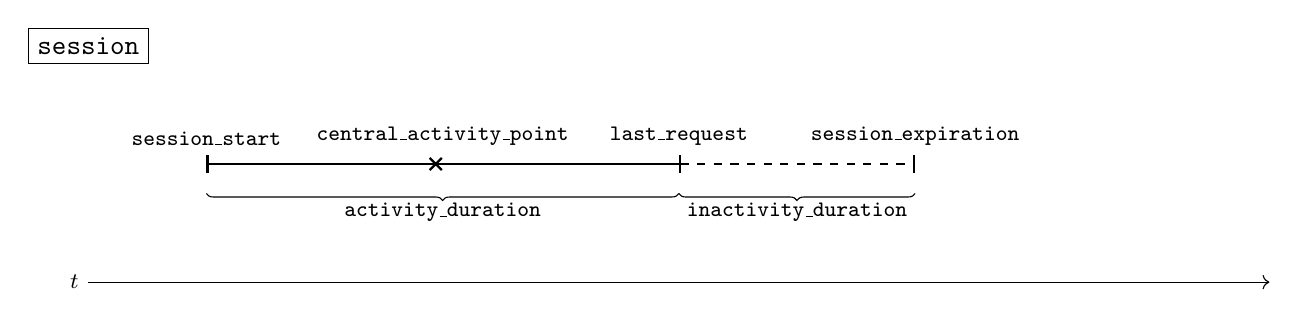
\begin{tikzpicture}[scale=1.5]

\tikzstyle{every node}=[font=\footnotesize]

\node (title) at (0,4) [font=\normalsize, draw] {\texttt{session}};

\draw[->] (0,2) node [left] {$t$} -- (10,2);
\draw[|-{Rays[]}, thick] 
			(1,3) node [above=3pt] 
				{\texttt{session\_start}} 
	-- 	(3,3) node [above=3pt] 
				{\texttt{central\_activity\_point}};
\draw[thick] (2.9,3) -- (5,3);
\draw[|-|, dashed, thick] 
			(5,3) node [above=3pt] 
					{\texttt{last\_request}} 
	-- 	(7,3) node [above=3pt] 
					{\texttt{session\_expiration}};

\draw[decorate,decoration={brace, mirror}]
			(1,2.75) -- (5,2.75) 
				node [midway,below] 
				{\texttt{activity\_duration}};
\draw[decorate,decoration={brace, mirror}]
			(5,2.75) -- (7,2.75) 
				node [midway,below] 
				{\texttt{inactivity\_duration}};
%\draw plot[mark=|] coordinates {(1,3) (3,3) (5,3) (7,3)};
%\draw plot[mark=|] coordinates {(1,3) (3,3) (5,3) (7,3)}; 
\end{tikzpicture}

\caption{
	\label{dia:session_structure}
	Diagrama del significat de cada un dels atributs pel que fa l'objecte \texttt{session}. 
}
\end{figure*}

Amb tot, noti's que a cada un dels usuaris que han establert les sessions de què tenim notícia, els quals són designats unívocament per mitjà de \texttt{user\_id}, li correspon un conjunt de sessions. Com és evident, doncs, podem prendre \texttt{user\_id} com a clau forània. En la figura \ref{dia:user_session_class} es mostra el senzill diagrama de classes que representa aquesta relació.

\begin{figure}
\begin{center}
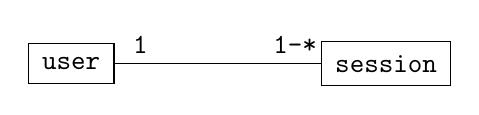
\begin{tikzpicture}[node distance=4cm]
\node (student) [draw, inner sep=5pt] {\texttt{user}};
\node (session) [draw, right of=student, inner sep=5pt] {\texttt{session}};
\draw (student) -- node [very near start, above] {\texttt{1}} node [very near end, above] {\texttt{1-*}}(session);
\end{tikzpicture}
\end{center}
\caption{
\label{dia:user_session_class}
	Diagrama de classes de la relació entre usuaris i sessions. 
}
\end{figure}

\subsection{Candidats de tipus objectes a modelar}

Després d'aquest primer cop d'ull, aturem-nos un moment a fer una llista de les classes d'objectes que podem abstraure a partir d'aquestes dades. La finalitat d'aquest exercici és donar un primer pas per a la concreció dels objectius del nostre estudi. 

\begin{enumerate}[(1)]

\item \textbf{Sessió}: Evidentment, en interpretar el contingut de \texttt{20131.con.txt} com una relació, ja estem considerant que les mateixes sessions són un possible objecte a modelar. De fet, podem considerar que són la classe primària que se'ns hi presenta, essent-ne les altres derivades.

\item \textbf{Cicles temporals}: Ja sigui per causes biològiques o socioculturals, el comportament dels humans presenta ritmes que segueixen cicles temporals. En aquest cas, estem considerant els humans que prenen part en el procés d'aprenentatge que té lloc en l'entorn educatiu del CV de la UOC. Per tant, aquestes unitats temporals poden ser un bon marc per a l'anàlisi de llur comportament. Podem identificar-ne, com a mínim, els següents:

	\begin{enumerate}[(a)]
	\item \textbf{Dia}, amb parts com les hores, matí, tarda, nit, etc. 
	\item \textbf{Setmana}, amb parts com els dies, laboral/festiu, etc.
	\item \textbf{Semestre}, és a dir, la totalitat del rang temporal en què es situen les dades rebudes. 
	\end{enumerate}
	
La caracterització d'aquests cicles vindrà donada, doncs, tant per la presència o absència de com per característiques de les sessions que corresponen a cada una de les seves parts.  

\item \textbf{Usuari}: Si, com hem dit, els usuaris són identificats per mitjà de \texttt{user\_id}, podem caracteritzar el comportament de cada un d'ells en funció dels dos tipus d'objectes anteriors, això és, de les sessions que ha establert i dels cicles temporals als quals aquestes pertanyen. 
 
\end{enumerate}

\subsection{Dimensions bàsiques}

Donem ara una idea general de les dimensions de les dades a tractar.  

El fitxer \texttt{20131.con.txt} en format text conté $661.17$ MB d'informació\footnote{En codificació de caràcters ASCII.} i consta de $8837062$ línies, que corresponen als casos que constitueixen la població del nostre estudi. 

Per altra banda, en la taula \ref{tab:vals_cardinality} s'indica quines són les cardinalitats dels respectius conjunts de valors diferents corresponents a cada un dels atributs de \texttt{session}. 

\begin{table}
\label{tab:vals_cardinality}
\begin{center}
\begin{tabular}{lr}
\toprule
atribut $a$ & $\left|\{x : x = \text{val}(a) \}\right|$ \\
\midrule
\texttt{id} & $8837062$ \\
\texttt{user\_id} & $75609$ \\
\texttt{session\_start} & $5059939$ \\
\texttt{last\_request} & $5072362$ \\
\texttt{session\_expiration} & $2135158$ \\
\bottomrule
\end{tabular}
\end{center}
\caption{
	Cardinalitat de valors distints que prenen cada un dels atributs dels objectes de la classe \texttt{session}.
}
\end{table}

Adverteixi's que les sessions han estat generades per part de $75608$ usuaris diferents.

En darrer lloc l'abast temporal de les dades és comprès entre els dos valors següents\footnote{Observi's que el format de les marques de temps que he utilitzat en aquest cas  no és pas el de les cadenes de text rebudes en el fitxer de dades, sinó l'estàndard ISO 8601. A fi de seguir la notació més comuna, a partir d'ara ho faré així.}:

\begin{align*}
\min(\texttt{session\_start}) &= \texttt{2013-09-18 00:00:03} \\
\max(\texttt{session\_expiration}) &= \texttt{2014-01-15 21:57:13} \\
\end{align*}

Com es pot veure, el rang temporal de les dades va des de la tercera setmana de setembre del 2013 fins a mitjans de gener del 2014. Aquest període de poc menys de $4$ mesos correspon de manera aproximada al desplegament temporal d'un semestre de tardor dels cursos ordinaris de la UOC.     
  
\section{Grau de coneixement del procés de generació de les dades}

Allò que ens interessa en un estudi com aquest no són les dades mateixes, sinó més aviat els esdeveniments que, en tenir lloc, n'han provocat l'aparició, a mode de rastres o indicis. És a causa d'aquest fet que es fa necessari interpretar-les. A l'hora de poder saber satisfactòriament quin n'és el significat, és a dir, quina informació proporcionen i en quina mesura ho fan, és especialment valuosa la recol·lecció del màxim de coneixement possible sobre el procés que les ha generades. 

Desafortunadament en realitat no he disposat de gaire més informació pel que fa aquesta qüestió que l'escueta descripció que ja s'ha proporcionat en la subsecció anterior. Sabem que cada una de les entrades del fitxer correspon unívocament a la sessió d'un usuari en el servidor del CV. D'aquest fet podem deduir, com a mínim, les següents conclusions:

\begin{enumerate}[(1)]

\item Atès que hom pot interactuar amb el CV de la UOC per mitjà d'un navegador web, algun tram de les connexions corresponents a part de les sessions establertes en la comunicació entre el client i el servidor ha tingut lloc per mitjà del \emph{Hypertext Transfer Protocol} (HTTP). 

\item Aquest és un protocol sense estat (\emph{stateless protocol})\citep[cap. 2]{kurose09}, és a dir, es tracta cada una de les transaccions\footnote{És a dir, cada un dels parells de petició-resposta presos com una unitat atòmica.} com quelcom independent d'aquelles que el mateix client ha iniciat anteriorment. Aquesta dificultat és sovint eludida per mitjà de galetes (\emph{cookies}) residents en el client, que l'identifiquen en cada transacció, o per mitjà de camps ocults en formularis enviats per mitjà del mètode \texttt{POST}.

\item Dels dos punts anteriors se'n dedueix, doncs, que \texttt{last\_request} tan sols indica quin és el segon en què el servidor del CV ha rebut la darrera petició per part del client que \texttt{user\_id} identifica. Noti's que això no implica que l'usuari que li correspon \emph{no hagi fet res}, en relació al procés d'aprenentatge, durant l'interval \texttt{inactivity\_duration}\footnote{Podria per, exemple, haver passat una bona estona llegint un document llarg}. En altres paraules, solament tenim notícia d'aquests dos moments d'interació entre client i servidor, però poca cosa més.   
\end{enumerate} 

En aquest sentit, és especialment rellevant tenir ben present \emph{quina informació no proporcionen} aquestes dades. Altrament, correríem el risc d'obtenir conclusions errònies tot construint arguments correctes a partir de suposicions infundades. Enumerem doncs quina és la informació que podríem caure en l'error de pensar que proporcionen però que en realitat no ho fan.

\begin{enumerate}[(1)]

\item En primer lloc, notem que no sabem res sobre el procés intern per mitjà del qual es recullen aquestes dades. És a dir, no sabem si consisteix en un \emph{log} escrit en temps real per part d'un servidor únic (o del node director d'un \emph{cluster}) o bé si són el resultat d'una agregació processada per lots (\emph{batch}) dels registres de nodes distints que executen instàncies diferents del programari del servidor del CV.

Tenim raons per a pensar que ens trobem en aquesta segon situació. Per exemple, en el cas que exposen Masip et al.\citep{massip10}, les dades d'accés al CV de la UOC són obtingudes a partir d'una combinació dels registres dels diferents servidors \emph{front-end} en què s'executa el programari que l'implementa. Aquesta combinació s'efectua per mitjà d'un procés per lots diàriament durant la matinada. Així, doncs, hem de comptar amb les particularitats d'un procés com aquest, en concret, amb la possibilitat de l'existència d'inconsistències en les dades.

\item D'altra banda, tampoc no sabem a quina mena d'usuari correspon cada un dels
identificadors. És a dir, si bé és correcte considerar que una part considerable dels identificadors d'usuari correspon a estudiants que es troben seguint un curs ordinari durant el semestre, no ho és pas suposar que ho fan tots. De fet, no podem suposar ni que són majoria. I és que cal tenir present que, a part d'estudiants, les sessions representades en les dades rebudes poden haver estat generades per part d'altres tipus d'usuaris. És raonable pensar, com a mínim, en els següents:

	\begin{enumerate}[(a)]
	\item Consultors, professors i altre personal docent.
	\item Personal purament acadèmic o de recerca.
	\item Membres de l'administració i serveis.
	\item Alumnes que no s'han matriculat en aquest semestre però que estan seguint alguns estudis a la UOC.
	\item Exalumnes de la UOC que, com a membres de \emph{UOC Alumni}, tinguin accés al CV.
	\item \emph{Bots} que estableixin sessions amb el servidor com a resultat de l'execució de tasques automàtiques.  
	\end{enumerate}
	
No hem rebut cap informació de part de l'organització del programa d'aquest treball de fi de grau (TFG) pel que fa aquest aspecte. L'única cosa que podem afirmar amb seguretat és que aquests usuaris són els agents d'aquestes sessions en el CV.

\item En tercer lloc, cal notar que tampoc tenim cap informació sobre quins són els fusos horaris a què corresponen els següents elements en joc:

	\begin{enumerate}[(a)]
	\item No coneixem el fus horari a definit en la configuració de cada un dels sistemes en què s'executa el programari que ha generat aquestes dades. 
	
	Suposaré, no obstant, que es tracta del mateix per a totes les entrades, a saber:
	$$
		\texttt{CET} = \texttt{UTC+01:00}
	$$
	
	\item No sabem tampoc quin és el fus horari corresponent la localització geogràfica des d'on ha tingut lloc la connexió per part de cada un dels usuaris que corresponen a clients controlats per humans, que han establert les sessions en cada cas. Ni tan sols disposem d'informació més general sobre aquest aspecte. En concret, no sabem quina és la proporció de sessions que s'estableixen des del fus \mt{CET}. 
	\end{enumerate}
	
Aquest fet provoca que tots els estudis d'anàlisi de dades referents al comportament de les sessions en funció del \emph{moment del dia} corrin el risc d'ésser considerablement esbiaixiats. Com es veurà tot seguit, he renunciat a emetre cap judici ferm en aquest sentit.  	

\end{enumerate}

\chapter{Neteja i transformació de dades}
\label{sec:data_anomalies}

En el marc del cicle de vida del KDD, el procés de tranformació i neteja de les dades en brut ha d'estar exclusivament al servei de l'objectiu que ens haguem proposat. Començarem, per tant, tot fent una descripició inicial de les dades rebudes. Aquesta consistirà, en primer lloc, en detectar-ne les possibles anomalies i considerar l'eliminació o normalització dels casos defectuosos. Seguidament reconeixerem quin dels seus trets poden suposar un obtacle per a assolir els nostres objectius i indicarem, si s'escau, quines són les transformacions adients per tal de superar-los. 

\subsection{Marques de temps incompletes}

D'entre les entrades del fitxer \texttt{20131.con.txt}, $370$ ($0.004 \%$) contenen, com a valor d'algun dels seus camps, una marca de temps que fretura de la indicació horària\footnote{És a dir, que segueix el patró ``\texttt{\%Y-\%m-\%d}''}. D'altra banda, no hi ha cap de les altres instàncies que presenti valors del tipus \mt{timestamp} que caiguin exactament en el segon \texttt{00:00:00}. Per tant, suposaré que en les primeres s'hi representa precisament aquest instant.

\subsection{Subsessions de durada negativa}

Si definim el conjunt: 
$$
 \mt{neg} =  \{v \in \texttt{sessions} : l(v.\mt{activity\_duration}) < \SI{0}{s} \vee 
    l(v.\mt{inactivity\_duration}) < \SI{0}{s} \}
$$  
aleshores $|\mt{neg}| = 467$ ($0.005\%$). El fet aparentment absurd que hi hagi parts de les sessions que constin com a tenint una durada negativa s'explica fonamentalment per dues causes. Exposem-les: 

\begin{enumerate}[(1)]
\item En $47$ dels elements de \mt{neg} és el cas que $l(\mt{activity\_duration}) < 0$. En totes elles tant \mt{session\_start} com \mt{last\_request} cauen entre les 2:00 i les 3:00 del matí del dia 27/10/2013, que és quan va tenir lloc, aquell any, el pas de l'horari d'estiu al d'hivern. Això no obstant, si bé resulta que aquesta duració negativa es deu a aquest canvi, \emph{això no significa que totes les distorsions introduïdes per part d'aquest canvi hagin provocat duracions negatives}. Poden donar-se, per exemple, situacions en què:

  \begin{enumerate}[(a)]
  \item Dues sessions constin com a simultànies i no ho siguin (sessions $v_0$ i $v_1$ de la figura \ref{dia:session_distortions}).
  
  \begin{figure}
  \begin{center}
  \begin{tikzpicture}[scale=1.5]

	\tikzstyle{every node}=[font=\footnotesize]

	\node (time) at (0,0) {$t$};
	\draw (time) -- (2,0);
	\draw[|-|] 
			(2,0) node [below=3pt] 
					{\mt{02:00}} 
	-- 	(4,0) node [below=3pt] 
					{\mt{02:00}$^\prime$};
	\draw[-|]
			(4,0) -- 	(6,0) node [below=3pt] 
					{\mt{03:00}};
	\draw[->] (6,0) -- (8,0);
	
	\draw[|-|, thick] (2.55, 1)  -- node[midway, below=3pt] {$v_0$} (3.85, 1);
	\draw[|-|, thick] (4.75, 1)  -- node[midway, below=3pt] {$v_1$} (5.75, 1);
	\draw[|-|, thick] (1.75, 0.5)  -- node[midway, below=3pt] {$v_2$} (6.35, 0.5);
	
  \end{tikzpicture}
  \end{center}
  \caption{
  	\label{dia:session_distortions}
		Exemples de distorsions introduïdes per part del canvi horari que no són detectables. 
  }
  \end{figure}
  
  \item Una sessió hagi començat abans de les 2:00 o hagi acabat després de les 3:00 y aquest fet la faci constar com havent durat una hora menys del que en realitat durà (sessió $v_2$ de la figura \ref{dia:session_distortions} ). 
  \end{enumerate}

Les sessions que compleixen la condició següent (és a dir, aquelles que són problemàtiques a causa d'aquest fet), són $1003$ ($0.01\%$):

\begin{align*}
	 (\texttt{session\_start} & \in [\texttt{2013-10-27 02:00:00}, \texttt{2013-10-27 03:00:00})) \\
  \vee & (\texttt{last\_request} \in [\texttt{2013-10-27 02:00:00},\texttt{2013-10-27 03:00:00})) \\
 \vee & (\texttt{session\_start} < \texttt{2013-10-27 02:00:00} \wedge \texttt{last\_request} < \texttt{2013-10-27 03:00:00}) \\
\end{align*}

Davant la impossibilitat de destriar les distorsions provocades per aquest fenomen i de les dades que en realitat són fiables, així com de l'escàs pes que tenen en la totalitat del conjunt de dades, he pres la decisió d'eliminar solament aquelles en què $l(\mt{activity\_duration})$ és negatiu, amb la finalitat de simplificar les operacions que es durant a terme més endavant. 

\item En $431$ casos (els conjunts definits per part de les dues condicions anteriors no són disjunts), el que s'ha esdevingut és que 
$$
	l(\texttt{inactivity\_duration}) < \SI{0}{\second}
$$
Això no obstant, en totes elles resulta que 
$$
	|l(\texttt{inactivity\_duration})| < \SI{5}{\second}
$$ 
i, de fet, en la majoria dels casos la diferència és solament d'un segon. Suposarem que això és causat per decalatges en l'arribada de peticions al servidor o, en general, a altres errors de funcionament intern. En aquests casos assumirem que 

$$
	\texttt{last\_request} = \texttt{session\_expiration}
$$

\item En darrer lloc, només hi ha una sessió amb subsessions de durada negativa que no s'expliqui per cap d'aquestes dues causes. Serà igualment eliminada.

\end{enumerate}


\chapter{Estadística descriptiva}

Atenguem-nos ara a la distribució dels valors dels diferents atributs dels objectes candidats a modelar que hem apuntat en la secció \ref{sec:natu_dades_rebudes}. Tot seguint el mateix ordre expositiu, començarem veient, de primer, les característiques de les sessions en general, de certs cicles temporals en segon lloc i, finalment, dels usuaris a què pertanyen. 

\section{Característiques dels atributs de les sessions}

Comencem donant un cop d'ull a la distribució dels diferents valors dels atributs de l'objecte \texttt{session}. En la taula \ref{tab:percentiles_sessions} es mostren els alguns dels percentils (100-quantils) dels valors dels atributs \texttt{activity\_duration} i \texttt{inactivity\_duration}. Observem-hi el següent:  

\begin{table*}
\begin{center}
\begin{tabular}{rrrrrr}
\toprule
100-quantil $k$-èssim   &
  $\lfloor k/100 \cdot |\texttt{sessions}| \rfloor$ &
   100-$q_{k\%}(l(\mt{a\_du}))$ &
   100-$q_{k\%}(l(\mt{ina\_du}))$ \\
\midrule
1 & 88365 & 0 & 0 \\ 
5 & 441829 & 3 & 0 \\ 
10 & 883659 & 9 & 0 \\ 
25 & 2209148 & 41 & 0 \\ 
50 & 4418297 & 203 & 4023 \\ 
75 & 6627446 & 1039 & 4049 \\ 
90 & 7952935 & 3401 & 4064 \\ 
95 & 8394765 & 5241 & 4074 \\ 
99 & 8748229 & 10869 & 4083 \\ 
\bottomrule \\
\end{tabular}
\end{center}
\caption{
	\label{tab:percentiles_sessions}
  Percentils rellevants dels valors dels atributs de \mt{session}. Els valors de les dues darreres columnes es mostren en segons. En la notació de les capçaleres $\mt{a\_du} = \mt{activity\_duration}$ i $\mt{ina\_du} = \mt{inactivity\_duration}$.  
}
\end{table*}

\begin{enumerate}[(1)]
\item Pel que fa \texttt{activity\_duration} la distribució dels valors és especialment desigual. La figura \ref{graph:activity_duration_dens} mostra una estimació de la funció de densitat de probabilitat (PDF) \citep{silverman86}\footnote[][\baselineskip]{Noti's addicionalment que aquesta estimació s'ha calculat en tots els casos mitjançant la funció \mt{density} del paquet base del programari R \citep{rteam14}, amb el nucli gaussià que empra per defecte.}. Observem dues característiques especialment rellevants en la distribució dels valors d'aquest atribut.
	\begin{enumerate}[(a)]
	\item En primer lloc la proporció de sessions amb una durada desmesuradament curta és notablement gran. A la taula \ref{tab:activity_duration_mins} es mostra el nombre de instàncies ($n_k$) i la freqüència ($f_k$) acumulades per a 6 $k$-valors de \mt{activity\_duration}. Tornarem a aquesta qüestió més endavant, però de moment noti's que un $30\%$ de les sessions presenten una duració d'activitat d'un minut o menys.
	
	\begin{figure}
    \begin{center}
    \includegraphics{activity_duration_a_dens}
    \end{center}
    \caption{
    \label{graph:activity_duration_dens}
    	Estimació de la PDF de \texttt{activity\_duration}
    }
  \end{figure}
	
	\item En segon lloc, val a dir que també presenta valors extrems per la dreta. Si bé el percentil 99 és a $\SI{10879}{\second}$ ($\SI{3.02}{h}$), noti's que a partir d'aquest punt els seus valors prenen valors desmesuradament alts. La taula \ref{tab:max_activity_duration_vals} mostra els $5$ valors més alts que pren aquest atribut.

	\end{enumerate} 
	
	\begin{margintable}
    \label{tab:activity_duration_mins}
    \begin{tabular}{rrr}
    \toprule
    $l(\mt{a\_du}) \leq k$ & $n_k$ & $f_k$ \\
    \midrule
    0 & 219359 & 2.5\% \\
    1 & 337924 & 3.8\% \\
    5 & 618676 & 7 \% \\
    10 & 979324 & 11.1 \% \\
    30 & 1872169 & 21.2 \% \\
    60 & 2681220 & 30.34 \% \\
    \bottomrule \\
    \end{tabular}
    
    \caption[]{
    Distribució dels valors més petits de $l(\mt{activity\_duration})$. Les abreviacions dels noms dels atributs són les mateixes que en la taula \ref{tab:percentiles_sessions}. Com es pot observar, La freqüència ($f_k$) s'expressa en percentatges.  
    }
  \end{margintable}
	
	\begin{margintable}
	\begin{center}
	\begin{tabular}{rr}
	\toprule
 	$i$ & $x_i$ \\
	\midrule
	\vdots & \vdots \\
	$n-4$ & 429742 \\
	$n-3$ & 512625 \\
	$n-2$ & 520141 \\
	$n-1$ & 562338 \\
	$n$   & 600528 \\ 
	\bottomrule \\
	\end{tabular}
	\end{center}
	\caption{
		\label{tab:max_activity_duration_vals}
		Els 5 valors més grans de \mt{activity\_durtation}.  
	}
	\end{margintable}

Podem mirar de prescindir d'aquests valors extrems i observar la distribució resultant si definim la condició $c$
	\begin{align*}
	c := & l(\mt{activity\_duration}) > \SI{60}{\second} \\
			& \wedge l(\mt{activity\_duration}) < 100\text{-}q_{95\%}(l(\mt{activity\_duration})) 
	\end{align*}
	i obtenim la relació $\mt{trim\_sessions} \subseteq \mt{sessions}$, de les tuples que la compleixen
	$$
	\mt{trim\_sessions} = \sigma_{c}(\mt{sessions})	
	$$
  Noti's que aleshores $|\mt{trim\_sessions}| = 5713445$ (el $64.5\%$ de la cardinalitat de \mt{sessions}).
  
  D'altra banda, en la figura \ref{graph:trim_activity_duration_dens} es mostra l'estimació de la PDF de \mt{trim\_sessions.activity\_duration}.
  
  \begin{figure}
  \begin{center}
  \includegraphics{trim_activity_duration_dens}
  \end{center}
  \caption{
  \label{graph:trim_activity_duration_dens}
  	Estimació de la densitat de probabilitat dels valors \mt{trim\_sessions.activity\_duration}
  }
  \end{figure} 

Observi's que, tot i que la taxa de decreixement de la probabilitat és menor, aquesta gràfica presenta un aspecte similar al de la figura \ref{graph:activity_duration_dens}. La moda de \mt{trim\_sessions.activity\_duration} en segueix essent el valor mínim i, per tant, el pic de la distribució es situa a $\SI{61}{s}$.   

\item La distribució del valors de \texttt{inactivity\_duration} és tota una altra. Com es pot veure en la taula \ref{tab:percentiles_sessions} el seu valor és $\SI{0}{s}$ fins a haver superat amb escreix el 25è percentil (recordi's que hem igualat a 0 les durades negatives en aquest cas). En la figura \ref{graph:inactivity_duration_dens} es mostra una estimació de la PDF dels valors d'aquest atribut. 

És fàcil reconèixer dos pics, que, de fet, divideixen les sessions en dues classes:

  \begin{enumerate}[(a)]
  
  \item La d'aquelles sessions que s'han tancat per mitjà de la sortida manual per part de l'usuari.
  
  \item La d'aquelles que han caducat automàticament després d'un temps estipulat en el programari del CV. Sembla que aquest temps ronda els $\SI{4008.2}{\second}$, que és la mitjana de la durada d'aquest atribut si prescindim dels valors nuls.
    
  \end{enumerate}

\end{enumerate}

\begin{figure}
\begin{center}
\includegraphics{inactivity_duration_a_dens}
\caption{
	\label{graph:inactivity_duration_dens}
	Estimació de la PDF de $l(\mt{inactivity\_duration})$. 
}
\end{center}
\end{figure}

\section{Descripció dels cicles temporals}

Analitzem tot seguit les distribucions de valors dels atributs dels objectes que corresponen als diferents cicles temporals que hem abstret en la secció \ref{sec:natu_dades_rebudes}.  

\subsection{El dia}

El primer d'aquests cicles temporals és del dia en què tenen lloc les diferents sessions\footnote{Les dades resultants dels resums d'aquesta subsecció es troben al fitxer \mt{session\_days.csv}}.

La gràfica present en la figura \ref{graph:student_session_hour_scatter} inclou les corbes corresponents a les dues variables següents:

\begin{enumerate}[(1)]
\item Per una banda, \mt{n\_sessions} representa el nombre de sessions que tenen \mt{central\_activity\_point} en l'hora del dia indicada per part de la variable independent com a proporció del màxim del seu rang, és a dir, com a percentatge de
 
$$
\max(|\{v \in \mt{sessions} : \mt{hour}(v.\mt{central\_activity\_point})= x\}|)
$$

on la funció \mt{hour} retorna l'hora del dia a què pertany un valor del tipus \mt{timestamp}.


\item Similarment, \mt{n\_users} expressa el nombre d'usuaris diferents que han establert sessions amb \mt{central\_activity\_point} igual al valor de l'eix de les abscisses també com a proporció del màxim del seu rang.   
\end{enumerate} 

\begin{figure}
\begin{center}
\includegraphics{student_session_hour_scatter}
\caption{
	\label{graph:student_session_hour_scatter}
	Proporció de sessions i usuaris per hora del dia en què s'esdevé \mt{central\_activity\_point}. 
}
\end{center}
\end{figure}

Les dues presenten uns trets generals similars:

\begin{enumerate}[(1)]
\item Hi veiem dos pics, un al voltant de les \SI{12}{\hour} i l'altre a l'entorn de l'intèrval $[\SI{18}{\hour}, \SI{20}{\hour}]$.
\item Per altra banda, dues valls, un mínim local a les $\SI{14}{\hour}$ i un d'absolut a les $\SI{4}{h}$.
\end{enumerate}

\begin{marginfigure}
\begin{center}
\includegraphics{c_a_point_h_bar}
\caption{
	\label{graph:c_a_point_h_bar}
	Nombre de sessions per hora del dia en què es dóna \texttt{central\_activity\_point}. 
}
\end{center}
\end{marginfigure}

\begin{marginfigure}
\begin{center}
\includegraphics{users_by_hour_bar}
\caption{
	\label{graph:users_by_hour_bar}
	Nombre d'usuaris únics de mitjana per hora del dia. 
}
\end{center}
\end{marginfigure} 

L'evolució que presenten els valors d'aquestes dues variables és completament compatible amb la idea que ens podríem haver format intuïtivament dels hàbits diaris de connexió dels estudiants de la UOC. Notem-ne el següent:

\begin{enumerate}[(1)]

\item En primer lloc, sembla que els dos punts de màxima activitat es troben a mig matí i a darrera hora de la tarda. Aquest esquema encaixa tant amb els estudiants que es dediquen a l'estudi a jornada completa i paren per dinar, com amb aquells que només hi dediquen o bé el matí o bé la tarda.

\item Per altra banda, el mínim absolut situat a les hores mitjes de la matinada encaixa amb la suposició segons la qual a aquestes hores la majoria d'estudiants estan dormint.

\item El desglossament d'aquestes variables en funció dels dies laborables i dels que pertanyen al cap de setmana no manifesta, no obstant, cap diferència notable respecte la totalitat dels casos. En els histogrames presents en les figures \ref{graph:student_session_hour_labdays} i \ref{graph:student_session_hour_weekend} se'n pot observar les distribucions respectives. 

Com es pot veure, l'evolució general és la mateixa. Ara bé, el cap de setmana, el màxim absolut pel que fa al nombre de sessions té lloc a la tarda, i el mínim relatiu de l'hora de dinar és més pronunciat.   

\begin{marginfigure}
\begin{center}
\includegraphics{student_session_hour_labdays}
\caption{
	\label{graph:student_session_hour_labdays}
	Proporció de sessions per hora del dia en què es dóna \texttt{central\_activity\_point} de dilluns a divendres. 
}
\end{center}
\end{marginfigure}

\begin{marginfigure}
\begin{center}
\includegraphics{student_session_hour_weekend}
\caption{
	\label{graph:student_session_hour_weekend}
	Proporció de sessions per hora del dia en què es dóna \texttt{central\_activity\_point} els caps de setmana. 
}
\end{center}
\end{marginfigure}

\item En darrer lloc hi ha un altre fet rellevant a tenir en compte que resulta d'aquesta distribució per hora del dia. En el capítol \ref{sec:data_anomalies} em referia a la manca d'informació sobre quin és el fus horari corresponent a la localització geogràfica del client que estableix la sessió en cada cas. La distribució dels valors de \mt{central\_activity\_point} en funció de l'hora del dia encaixen amb el patró dels ritmes diaris que hom pot observar, com a mínim, en els llocs geogràfics següents:
 
 \begin{enumerate}
 
 \item Pel que fa el fus \mt{CET}$=$\mt{UTC+01:00}, és coherent aquella que podem observar a l'Estat Espanyol. Pel que sé, als altres territoris que hi pertanyen tant els àpats com el moment de descans nocturn acostuma a tenir lloc una o dues hores abans.
 
 \item També encaixa amb els ritmes propis dels territoris europeus que es troben situats en el fus \mt{WET}$=$\mt{UTC+00:00}, ja que el ritme diari també és desfasat una o dues hores abans en relació a l'espanyol.
  
 \end{enumerate}
 
 Certament, desconeixem quina és la proporció d'usuaris del CV que resideixen habitualment al Regne Unit, Irlanda o Portugal, d'entre aquells que ho fan a l'estranger. Si no en són una part extraordinàriament gran, aleshores es pot concloure que en realitat la gran majoria s'hi connecten des de territori espanyol.  
   
\end{enumerate}

\subsection{La setmana}

Observem tot seguit el comportament de les mateixes variables en funció dels dies de la setmana (figura \ref{graph:student_session_wday_scatter})\footnote{Les dades resultants dels resums d'aquesta subsecció es troben al fitxer \mt{session\_weeks.csv}}.

\begin{figure}
\begin{center}
\includegraphics{student_session_wday_scatter}
\caption{
	\label{graph:student_session_wday_scatter}
	Nombre de sessions per dia de la setmana què es dóna \texttt{central\_activity\_point}. 
}
\end{center}
\end{figure}  

Altra vegada, les dues corbes presenten una estructura similar tot i que en aquest cas el nombre de per dia de la setmana presenti trets més accentuats. Com també podríem haver suposat \emph{a priori}, tant aquest valor com el d'usuaris únics davalla durant el cap de setmana, essent el dissabte el dia amb menys activitat. 

Per a una distribució en nombres absoluts de les variables consulti's els histogrames respectius de les figures \ref{graph:sessions_wday_bar} i \ref{graph:users_wday_bar}.


\begin{marginfigure}
\begin{center}
\includegraphics{sessions_wday_bar}
\caption{
	\label{graph:sessions_wday_bar}
	Nombre de sessions per dia de la setmana què es dóna \texttt{central\_activity\_point}. 
}
\end{center}
\end{marginfigure}

\begin{marginfigure}
\begin{center}
\includegraphics{users_wday_bar}
\caption{
	\label{graph:users_wday_bar}
	Nombre d'usuaris únics per dia de la setmana. 
}
\end{center}
\end{marginfigure} 

La interpretació de la diferència entre els comportaments de les dues variables té a veure amb el fenomen que ja hem observat en la subsecció anterior sobre els comportaments horaris que presenten en dies laborables (figura \ref{graph:student_session_hour_labdays}) i el cap de setmana (figura \ref{graph:student_session_hour_weekend}), respectivament. És raonable creure que hi ha una proporció considerable d'usuaris que tot i que segeuixen visitant el CV durant el cap de setmana (tal com havien fet durant els dies laborables), en aquest cas ho fan amb menys intensitat. 

\subsection{El semestre}

Completem ara la nostra inspecció inicial dels cicles temporals tot atenent-nos al semestre en la seva totalitat\footnote{Les dades resultants dels resums d'aquesta subsecció es troben al fitxer \mt{session\_semester.csv}}. Això consisteix en posar la nostra atenció en les característiques de les seves diferents parts en funció de la presència o absència de sessions i/o usuaris, i dels trets que aquestes presenten. 

Per a fer-ho, observem els resultats que s'exposen en les gràfiques de les figures \ref{graph:n_sessions_pday_scatter} i \ref{graph:n_users_pday_scatter}, respectivament. Hi trobem un diagrama de punts i línies que relaciona el dia del semestre amb cada una de les dues variables que hem vingut observant fins ara. En el primer cas, les ordenades indiquen el nombre de sessions l'atribut \mt{central\_activity\_point} de les quals cau en la data que correspon al valor de la variable independent. En el segon allò que indica la variable dependent és el nombre d'usuaris únics que són els agents d'aquestes sessions.

En tots dos casos, els punts mostren els valors obtinguts i la línia grisa fa palesa llur precedència cronològica. A més, com es pot veure, el color dels punts indica el dia de a setmana a què corresponen. En darrer lloc, noti's que en tots tres casos també s'hi ha sobreimprès, en color blau, la corba resultant de l'aplicació de la regressió local (LOESS) \citep{cleveland79}\footnote{El càlcul concret d'aquesta regressió no paramètrica s'ha dut a terme per mitjà de la funció \mt{loess} del paquet \mt{stats} de programari R \citep{rteam14}}, envoltada d'una zona ombrejada que representa l'evolució de l'amplada de l'interval de confiança.     

\begin{figure}
\begin{center}
\includegraphics{n_sessions_pday_scatter}
\caption{
	\label{graph:n_sessions_pday_scatter}
	Nombre de sessions per dia del semestre. El color dels punts indica el dia de la setmana de què es tracta. 
}
\end{center}
\end{figure}

\begin{figure}
\begin{center}
\includegraphics{n_users_pday_scatter}
\caption{	
	\label{graph:n_users_pday_scatter}
	Nombre d'usuaris únics per dia del semestre. El color dels punts indica el dia de la setmana de què es tracta. 
}
\end{center}
\end{figure}

Dels dos resultats, cal notar-ne el següent:

\begin{enumerate}[(1)]

\item La dispersió dels valors s'explica per la variació del dia de la setmana a què pertanyen, la qual esdevé una raó suficient per a haver-nos plantejat la setmana com una unitat temporal digna d'interès, tal com hem fet en la secció \ref{sec:natu_dades_rebudes}. Si parem atenció al cicle $[\mt{dl}, \mt{dg}]$, veurem que, en quasi tots els casos, las distribució dels valors és coherent amb els resultats setmanals que es mostren en la gràfica de la figura \ref{graph:student_session_wday_scatter}. La regularitat d'aquest patró només es trenca a partir de la darrera setmana de desembre, que és el moment en què comencen les festes de Nadal, durant les quals és raonable pensar que s'alteren els hàbits diaris dels usuaris. 

\item En tots dos casos la corba de la LOESS mostra una tendència similar. Podem distingir-hi els tres trams següents:

	\begin{enumerate}[(a)]
	\item Un primer tram d'evolució tímidament creixent des de l'inici de curs fins a primers de novembre.
	\item Un de segon que ocupa tot el novembre. Tot i que en general el pendent és negatiu és tant a prop del zero que el podem veure com un altiplà amb un lleu mínim local.
	\item Un darrer tram que s'inicia amb l'entrada del desembre i que presenta un decreixement accelerat fins al final del semestre.  
	\end{enumerate}

Tot i que en tot moment hem de tenir present que no sabem del cert quina és la proporcio d'usuaris que són estudiants, llur comportament general també és coherent amb la imatge preconcebuda que ens proporciona el sentit comú sobre quina és l'evolució de la relació que mantenen amb l'activitat acadèmica que segueixen i, per tant, amb el CV. Pel que fa l'esquema general preconcebut sobre l'evolució del curs acadèmic, podem interpretar així els tres trams que acabem d'identificar:

	\begin{enumerate}[(a)]
	\item El primer tram consisteix en un \emph{període d'incorporació} dels estudiants. Ja sigui perquè n'hi ha que no inverteixen una gran dedicació a l'estudi just a principi de curs, perquè sempre es deixa un temps prudencial fins el lliurament de la primera \emph{Prova d'Avaluació Continuada} (PAC) o perquè n'hi ha que, fruit d'una ampliació de matrícula, amplien la presència al CV, durant aquest tram l'activitat augmenta progressivament. 
	  
	\item En el segon hi trobem un \emph{màxim d'activitat}. Així doncs, consisteix en el nucli del curs, on la suma de la dedicació de tots els estudiants és la més alta.
	
	\item En el tercer hi podem identificar el que podríem anomenar com un \emph{període de garbellat i clausura}. En aquest cas, tots aquells estudiants que, per les raons que sigui, ja tenen clar que no superaran una part o la totalitat de les assignatures a què estan matriculats, redueixen la seva activitat al CV o l'abandonen completament. Cal tenir present, no obstant, que durant el període comprès entre la segona setmana de gener i el final de semestre l'activitat acadèmica no exigeix una atenció constant al CV fins i tot per a aquells estudiants que han seguit el curs satisfactòriament.      
	\end{enumerate}
\end{enumerate}

\section{Característiques dels atributs dels usuaris}
\label{sec:user_stats}

Per a tancar aquesta secció mirem de fer un estudi preeliminar sobre el darrer dels objectes a modelar que hem apuntat en la secció \ref{sec:natu_dades_rebudes}, a saber, els usuaris, que representarem per mitjà de l'objecte \mt{user}\footnote{Les dades resultants dels resums d'aquesta subsecció es troben al fitxer \mt{users.csv}}. Com fa palès, aquest és un objecte derivat. Denotarem l'esquema de la classe que els defineix de la manera següent:

\begin{fullwidth}
$$
\mt{user(user\_id, n\_sess, sum\_a\_du, m\_a\_du, m\_wday, m\_hour, f\_sess, l\_sess)}
$$
\end{fullwidth}

Per a cada valor distint $i$-èssim de l'atribut \mt{user\_id} de \mt{session}, construirem doncs un objecte $\mt{user}_i$ els valors dels atributs del qual calcularem com s'indica a continuació. Sigui 
$$
	\mt{sessions}_i := \sigma_{(\mt{user\_id} = \mt{user\_id}_i)}(sessions)
$$ 
Aleshores hi definim els atributs següents:

\begin{fullwidth}
\begin{enumerate}[(1)]

\item $
\mt{id}_i := \mt{user\_id}_i \in  ([\mt{``0''}, \mt{``9''}] \cup \{`` ''\}){13}
$

\item $
\mt{n\_sess}_i := 
	|\mt{sessions}_i| \in \mathbb{N}
	$
	
\item 
$ \displaystyle
\mt{sum\_a\_du}_i := 
	\sum_{v \in \mt{sessions}_i} l(v.\mt{activity\_duration}) \in \mathbb{N}\times \SI{}{\second}
$

\item $ \displaystyle
\mt{m\_a\_du}_i := \frac{\mt{sum\_a\_du}_i}{\mt{n\_sess}_i} \in \mathbb{R} \times \SI{}{\second} 
$

\item $ 
\mt{m\_wday}_i := 
\displaystyle
	\frac{
		1
	}{
		 \mt{n\_sess}_i
	} 
	\displaystyle	\sum_{v \in \mt{sessions}_i} 
				\mt{wday}(v.\mt{central\_activity\_point})
	\in [0,6] \subseteq \mathbb{R}$
			
\item $
	\mt{m\_hour}_i := 
	\displaystyle
	\frac{1}{\mt{n\_sess}_i}
	\displaystyle
	\sum_{v \in \mt{sessions}_i} 
			\mt{hour}(v.\mt{central\_activity\_point})  \in [0,23] \subseteq \mathbb{N}$ 
			
\item $\mt{f\_sess}_i := 
	\min(\{ v.\mt{central\_activity\_point} : v \in \mt{sessions}_i\}) \in \mt{timestamp} $ 
	
\item $\mt{l\_sess}_i := 
	\max(\{ v.\mt{central\_activity\_point} : v \in \mt{sessions}_i\}) \in \mt{timestamp} $ 
			
\end{enumerate}
\end{fullwidth}

Com es pot observar, de moment ens hem centrat fonamentalment en dos aspectes de la relació entre els usuaris i les sessions que han establert.

\begin{enumerate}[(1)]

\item En les mitjanes mostrals dels valors dels atributs de les sessions que corresponen a cada usuari.

\item En la durada de l'activitat de cada usuari, delimitada pels valors \mt{central\_activity\_point} corresponents a les seves primera i darrera sessions.
 
\end{enumerate}
 Anomenarem \mt{users} la relació que conté tots els casos de \mt{user} obtinguts, la qual, recordem, presenta la següent cardinalitat:

$$
 |\mt{users}| = 75609
$$

\subsection{Distribució dels valors de les mitjanes mostrals}

Una simple inspecció de certs percentils dels valors que prenen les mitjanes mostrals que dónen valor a $5$ atributs d'aquest nou objecte ens permet copsar ràpidament que en aquest cas també presenten una disparitat molt acusada. En tenim una mostra en la taula \ref{tab:users_desc}.  
  
\begin{table*}
\begin{center}
\begin{tabular}{rrrrrrr}
\toprule
100-quantil &
  $\lfloor k/100 \cdot |\texttt{users}| \rfloor$ &
   \mt{n\_sessions} &
   \mt{sum\_a\_du} &
   \mt{m\_a\_du} &
   \mt{m\_wday} &
   \mt{m\_hour} \\
\midrule
 1 &   756 &   1 &      28 &   18.5 & 0.00 &  6.0 \\ 
 5 &  3780 &   1 &     185 &   90.6 & 1.00 & 10.5 \\ 
10 &  7560 &   2 &     488 &  167.4 & 1.75 & 11.9 \\ 
25 & 18902 &   7 &    3674 &  383.6 & 2.24 & 13.5 \\ 
50 & 37804 &  68 &   47500 &  749.0 & 2.64 & 14.8 \\ 
75 & 56706 & 167 &  161972 & 1248.9 & 3.00 & 16.1 \\ 
90 & 68048 & 296 &  341317 & 1814.9 & 3.50 & 17.6 \\ 
95 & 71828 & 399 &  515577 & 2252.9 & 4.00 & 19.0 \\ 
99 & 74852 & 670 & 1087294 & 3785.7 & 6.00 & 22.0 \\ \bottomrule \\
\end{tabular}
\end{center}
\caption{
	\label{tab:users_desc}
	Percentils rellevants dels valors numèrics de \mt{user}.
}
\end{table*}

De fet, en \mt{n\_sessions}, \mt{sum\_a\_du} i \mt{m\_a\_du}, hi ha tants valors petits i tenen valors molt alts un nombre tan petit de casos que moltes de les representacions gràfiques que en poguem fer són de poca utilitat. Llurs distribucions presenten un rang interquartílic tan petit en relació als valors més elevats que en un diagrama de caixes aquestes se'n apareixerien com un segment horitzonal. Per altra banda, una gràfica de l'estimació de la PDF d'alguns d'ells tindria un aspecte encara més similar a una ``L'' del que es pot apreciar en la corba de la gràfica de la figura\ref{graph:activity_duration_dens}. És per aquesta raó que representarem aquesta distribució mitjancant corbes d'estimació de la densitat de probabilitat en gràfiques l'escala de les abscisses de les quals sigui logarítmica en base 10.

\begin{margintable}
    \begin{tabular}{rrr}
    \toprule
    $\mt{n\_sess} \leq k$ & $n_k$ & $f_k$ \\
    \midrule
    1 & 6880 & 9 \% \\
    2 & 10978 & 13.5 \% \\
    3 & 13704 & 18.1 \% \\
    4 & 15542 & 20.5 \% \\
    5 & 17030 & 22.5 \% \\
    \bottomrule \\
    \end{tabular}
    
    \caption[]{
    \label{tab:n_sess_mins}
    Distribució dels valors més petits de \mt{n\_sess}. Com es pot observar, la freqüència acumulada ($f_k$) s'expressa en percentatges.  
    }
  \end{margintable} 

En primer lloc, en la figura \ref{graph:user_n_sessions_density_line_log} hi podem trobar una representació d'aquesta mena pel que fa els valors de \mt{n\_sess}. Podem observar-hi com el gruix dels usuaris del CV han establert un nombre de sessions que ronda les 100. 

\begin{figure}
\begin{center}
\includegraphics{user_n_sessions_density_line_log}
\caption{
	\label{graph:user_n_sessions_density_line_log}
	Estimació de la PDF dels valors de l'atribut \mt{n\_sess}. L'escala de les abscisses és logarítmica en base 10. 
}
\end{center}
\end{figure}

\begin{margintable}
	\begin{center}
	\begin{tabular}{rr}
	\toprule
 	$i$ & $x_i$ \\
	\midrule
	\vdots & \vdots \\
	$n-4$ & 3346 \\
	$n-3$ & 3698 \\
	$n-2$ & 3730 \\
	$n-1$ & 5408 \\
	$n$   & 65160 \\ 
	\bottomrule \\
	\end{tabular}
	\end{center}
	\caption{
		\label{tab:max_n_session_vals}
		Els 5 valors més grans de \mt{n\_sessions}.  
	}
	\end{margintable} 

El fenomen que sí que mereix especial atenció és, no obstant, l'acumulació de valors molt a prop de l'$1$. La taula \ref{tab:n_sess_mins} mostra el nombre d'observacions i la freqüència corresponents als cinc valors més petits de \mt{n\_sess}. És rellevant constatar com el 9\% de tots els usuaris només han establert una sessió amb el CV, així com quasi una quarta part només n'han establert 5 o menys. Per altra banda, si bé el percentil 99è d'aquest atribut es situa a 670 sessions, a partir d'aquest punt els valors es disparen molt ràpidament. En la taula \ref{tab:max_n_session_vals} es mostren els 5 valors més grans que pren.

La distribució dels valors també presenta una gran disparitat si ens atenem a l'atribut \mt{sum\_a\_dur}, això és, a la suma total dels segons en què l'usuari ha estat actiu. La gràfica de la figura \ref{graph:user_n_sessions_density_line_log} mostra la corba de l'estimació de la PDF per als valors d'aquest atribut, també amb una escala logarítmica en l'eix de les abscisses.    

\begin{figure}
\begin{center}
\includegraphics{user_sum_activity_duration_density_line_log}
\caption{
	\label{graph:user_sum_activity_duration_density_line_log}
	Estimació de la PDF dels valors de l'atribut \mt{sum\_a\_du}. L'escala de les abscisses és logarítmica en base 10. 
}
\end{center}
\end{figure}

A primer cop d'ull, la dispersió en la franja alta els valors no sembla tan acusada com en el cas anterior. Observem que el gruix dels usuaris han presentat, en segons, una durada total de l'activitat en l'interval $[10^2,10^{5.5}]$\footnote{Noti's que aquest interval és, igualment, molt gran.}, amb un màxim al voltant de $10^5$ ($\SI{2.7}{\hour}$). Ara bé, aquesta aparença és causada en efecte per la transformació logarítmica que hem introduït en l'escala de la variable independent. En la gràfica de la figura \ref{graph:user_sum_activity_duration_density_line}, en què l'escala és lineal, amb prou feines es pot apreciar a simple vista l'àrea compresa sota la línia que hi apareix.   

\begin{marginfigure}
\begin{center}
\includegraphics{user_sum_activity_duration_density_line}
\caption{
	\label{graph:user_sum_activity_duration_density_line}
	Estimació de la PDF per a \mt{sum\_activity\_duration}. 
}
\end{center}
\end{marginfigure}

Val a dir que en aquest cas la causa de la gran disparitat observable recau en major mesura en els valors extrems, que són els que provoquen que la cua de la dreta sigui tan llarga. La informació present en les taules \ref{tab:sum_a_du_mins} i \ref{tab:max_sum_a_du_vals} dona fe d'aquest fet.    

\begin{margintable}
    \begin{tabular}{rrr}
    \toprule
    $\mt{sum\_a\_du} \leq k$ & $n_k$ & $f_k$ \\
    \midrule
    0 & 234 & 0.3 \% \\
    1 & 374 & 0.5 \% \\
    30 & 796 & 1 \% \\
    60 & 1362 & 1.8 \% \\
    600 & 8506 & 11.3 \% \\
    1800 & 14558 & 19.3 \% \\
    3600 & 18763 & 24.8 \% \\
    \bottomrule \\
    \end{tabular}
    
    \caption[]{
     \label{tab:sum_a_du_mins}
    Distribució dels certs valors de \mt{sum\_a\_du}. Com es pot observar, la freqüència acumulada ($f$) s'expressa en percentatges.  
    }
  \end{margintable} 
  
\begin{margintable}
	\begin{center}
	\begin{tabular}{rr}
	\toprule
 	$i$ & $x_i$ \\
	\midrule
	\vdots & \vdots \\
	$n-4$ & 3346 \\
	$n-3$ & 3698 \\
	$n-2$ & 3730 \\
	$n-1$ & 5408 \\
	$n$   & 65160 \\ 
	\bottomrule \\
	\end{tabular}
	\end{center}
	\caption{
		\label{tab:max_sum_a_du_vals}
		Els 5 valors més grans de \mt{sum\_a\_du}.  
	}
	\end{margintable}


Això no obstant, la conclusió útil que podem extreure dels trets del comportament d'aquestes dues variables és quelcom prou concret. Les distribucion respectives dels valors d'aquests dos atributs són una raó suficient per a no descartar la hipòtesi segons la qual la proporció d'usuaris que no corresponen a estudiants matriculats en un curs ordinari de la UOC és considerable. Observem sinó el següent:

\begin{enumerate}[(1)]

\item És raonable pensar que un estudiant es connectarà 5 vegades o més al CV pel cap baix. Cal tenir present que, per a seguir satisfactòriament el curs com a mínim a de realitzar tasques com llegir el pla docent a l'inici del semestre, presentar tres o més PACs, consultar els horaris dels exàmens, etc.

\item També és raonable considerar que la suma del temps necessari per a dur a terme les accions que s'enumeren en el punt anterior és com a mínim d'una hora. 

\end{enumerate}   

Noti's que hi ha gairebé $1/4$ dels usuaris que no satisfan les dues condicions que s'acaben d'apuntar. Ara bé, no gosaré intentar estimar quina és la proporció d'usuaris que corresponen a estudiants, ja que entenc que, amb les dades de què disposem, aquesta tasca no és factible dins d'uns intervals de confiança raonables. En el capítol següent (\ref{chap:metrics_utility}) donaré més raons per a defensar aquesta tesi. Limitem-nos de moment a corroborar la nostra sospita sobre la diversitat d'usuaris que s'amaquen rere els identificadors de l'atribut \mt{session.user\_id}. 

\subsection{Relació entre la primera i darrera sessions}

Tancarem aquesta secció tot posant la nostra atenció en la informació que podem obtenir a partir de l'estudi de les relacions entre els dos punts temporals en què tenen lloc la primera i la darrera sessions de cada usuari (atributs \mt{f\_sess} i \mt{l\_sess}).

En primer lloc, notem que l'interval temporal comprès entre \mt{f\_sess} i \mt{l\_sess} és una bona representació del període en què l'usuari ha estat actiu pel que fa la seva relació amb el CV de la UOC. Hi ha, com a mínim, dues dimensions interessants d'aquest interval:

\begin{enumerate}[(1)]

\item La \emph{mida} de l'interval, és a dir:
	$$
	l([\mt{f\_sess}, \mt{l\_sess}])
	$$
	
\item La \emph{seva posició} en el desenvolupament temporal del semestre. És a dir, allà on caigui el valor central del periode d'activitat, que podem definir 
	$$
		(\mt{f\_sess} + l([\mt{f\_sess}, \mt{l\_sess}])) / 2
	$$
\end{enumerate} 

Una bona manera de mostrar la distribució dels usuaris en funció d'aquests dos paràmetres és l'elaboració d'un diagrama de dispersió com el que es mostra en la figura \ref{graph:user_first_last_scatter}. Noti's que cada punt representa un usuari, en què la seva posició en l'eix de les abscisses correspon al valor de \mt{l\_sess} i la del de les ordenades al de \mt{f\_sess}.  

\begin{figure*}
\begin{center}
\includegraphics[width=14cm]{user_first_last_scatter}
\caption{
	\label{graph:user_first_last_scatter}
	Diagrama de dispersió que relaciona els valors de \mt{f\_sess} i \mt{l\_sess}
}
\end{center}
\end{figure*}

Aquesta gràfica proporciona molta informació útil per als nostres objectius. En primer lloc, notis que la diagonal \emph{perpedicular} a la recta $y = x$ és una bona magnitud per a representar la mida de l'interval d'activitat de cada usuari. És a dir, com més lluny es trobi un punt de la recta $y  = x$, més gran és la distància temporal que hi ha entre les seves primera i darrera sessions.

Per que fa la distribució dels casos, observem el següent:

\begin{enumerate}[(1)]  

\item La gran acumulació de casos en la cantonada inferior dreta de la gràfica correspon a aquells usuaris que començaren la seva activitat al CV d'hora, en el desenvolupament del semestre i l'acabaren tard. És raonable incloure aquí que tots aquells usuaris que són estudiants i que han seguit un curs ordinari en la seva totalitat. Tot i això, és important tenir present que aquesta premissa no implica que en siguin la majoria.

\item La zona fosca en forma triangular que trobem en la cantonada superior dreta està composta per tots aquells usuaris que es connectaren tard per primera vegada. Sembla que el seu pes no és menyspreable. 

\item La gran concentració de casos que ressegueixen la recta $y = x$ correspon al considerable grup d'usuaris als quals només els correspon una sessió o que, si més no, presenten un interval d'activitat semestral extremadament curt.

\item La franja vertical de punts que es dibuixa a cavall del primer i segon quarts del més de gener en l'eix de les abscisses correspon a aquells usuaris que van connectar-se per primera vegada passat el primer d'octubre, però el període d'activitat del qual abasta fins després de les vacances de Nadal. Aquesta columna presenta una densitat decreixent en sentit vertical, cosa que és completament coherent amb el fet que per a aquells estudiants que encara no han començat a dedicar-se al curs al qual s'han matriculat, com més temps passa, més difícil és que puguin superar-lo i, per tant, menys probable és que ho facin. No obstant això, cal no oblidar en cap moment que això tampoc no indica res pel que fa la proporció d'usuaris inclosos en aquesta franja que corresponen a estudiants. Per altra banda, notis que s'hi dóna un patro d'alternança. Això encaixa completament amb les davallades d'activitat que s'observen durant el cap de setmana, tal com es pot veure en els resultats que s'exposen en la secció anterior.

\item En darrer terme, observi's que també es pot apreciar una franja horitzontal, en aquest cas més estreta, a l'alçada de la primera setmana del curs de l'eix de les ordenades. Noti's que presenta una gradació creixent en la seva densitat. No és forassenyat suposar que aquesta correspon a un altre comportament que a què apunta el sentit comú pel que fa els estudiants d'un curs ordinari, a saber, que a mesura que passa el temps n'augmenta el nombre que l'abandona.
      
\end{enumerate}

Aquests resultats són els primers que ens poden fer pensar que hi ha la possibilitat de descobrir tipologies d'usuaris per mitjà de mètodes d'agregació (\emph{clustering}) que siguin útils per als nostres propòsits, així com també en la utilitat de l'aplicació d'algoritmes d'aprenentatge computacional supervisat per tal d'obtenir alguna classificació reeixida i, si s'escau, predir-ne certes característiques. Fins a quin grau és possible fer això i quines serien les transformacions addicionals de les dades necessàries per a realitzar aquestes tasques és el que s'exposa en el capítol següent.   

      
\chapter{Consideració sobre la densitat semàntica de les variables}
\label{chap:metrics_utility}

Després d'haver fet una primera ullada a les característiques dels valors d'alguns dels atributs dels objectes bàsics que s'han definit en la secció \ref{sec:natu_dades_rebudes}, és un bon moment ara per a mirar d'escatir fins a quin punt aquests poden esdevenir una font de coneixement que ens sigui útil per la consecució dels nostres objectius.  

\section{Utilitat dels atributs emprats}
\label{sec:metrics_utility}

Tinguem present que, com s'ha enunciat en la secció \ref{sec:natu_dades_rebudes}, la finalitat, en aquest estudi, de l'aplicació del mètodes propis del KDD i l'ML en les dades rebudes ha d'ésser la de proporcionar-nos un coneixement que sigui útil per a, en darrera instància, millorar els processos d'aprenentatge en general i, en concret, aquells que es donen en el marc del CV de la UOC. Així doncs, no és sobrer preguntar-se fins a quin punt poden ajudar-nos en aquesta direcció els valors dels atributs dels objectes construïts a partir de l'abstracció elemental que s'ha fet fins ara. Com em sembla haver provat en la segona part de la secció que ara s'enceta, la resposta a aquesta qüestió és que,  sense cap transformació ulterior, l'ajuda que ens brinden és virtualment nul·la.

Això no obstant, com a part del desenvolupament del meu argument, caldrà primer aturar-se en la descripció d'una carcaterística de les dades rebudes que encara no s'ha esmentat i que suposaria un obstacle addicional per l'assoliment dels nostres objectius si no introduíssim les transformacions que proposo a continuació.   

\subsection{Solapament de sessions}

Un estudi una mica més exhaustiu de les dades que s'han rebut ens permet descobrir que hi ha sessions distintes corresponents a un mateix \texttt{user\_id} els respectius intervals \texttt{activity\_duration} de les quals es solapen. Resseguim l'operació en àlgebra relacional \citep{codd70} que ens permet obtenir aquest resultat. En primer lloc, definim, per a cada usuari $\mt{user\_id} \in \mt{users}$ les relacions següents:

\begin{fullwidth}
  \begin{align*}
  \mt{sessions}_i & := \pi_{(\mt{id},
                                    \mt{session\_start},
                                    \mt{last\_request})}( 
                \sigma_{(\mt{user\_id}=\mt{id}_i)}(
                    \mt{sessions})) \\
  \texttt{sessions\_0}_i & 
      := \rho_{(\mt{id\_0} / \mt{id}, 
                \mt{session\_start\_0}/\mt{session\_start},
                \mt{last\_request\_0}/\mt{last\_request})}(
            \mt{user\_sessions}_i) \\
  \mt{sessions\_1}_i & 
      := \rho_{(\mt{id\_1} / \mt{id\_0}, 
                \mt{session\_start\_1}/\mt{session\_start\_0},
                \mt{last\_request\_1}/\mt{last\_request\_0})}(
              \mt{user\_sessions\_0}_i) \\
  \end{align*}
\end{fullwidth}

Emprant els noms dels atributs de les dues darreres noves relacions, que són la mateixa duplicada, definim ara la condició $c$ de la manera següent: 

\begin{align*}
c := & (\mt{id\_0} < \mt{id\_1}) \wedge (\mt{session\_start\_0} \leq \mt{last\_request\_1}) \wedge  (\mt{session\_start\_1} \leq \mt{last\_request\_0}) \\
\end{align*}

Noti's que els dos darrers termes d'aquesta conjunció conformen la condició necessària per a poder afirmar que els dos intervals 

\begin{align*}
	[\mt{session\_start\_0}, & \mt{last\_request\_0}] \\
	[\mt{session\_start\_1}, & \mt{last\_request\_1}]
\end{align*} 

es solapen. Per altra banda, el primer, $(\mt{id\_0} < \mt{id\_1})$, té la finalitat d'evitar que en la relació resultant de la $(<)$-combinació que s'indica a continuació es compti un mateix solapament més d'un cop o s'hi inclogui el d'una sessió amb ella mateixa.  
 
En darrer lloc, obtenim la relació \mt{overlappings} tot definint-la així:

\begin{align*}
\mt{overlappings} := \bigcup_{i} \left( \mt{user\_sessions\_0}_i \bowtie_{c} \mt{user\_sessions\_1}_i \right) 
\end{align*}

És a dir, mitjançant la unió de totes les relacions que s'han obtingut per a cada un dels usuaris. Aquesta relació conté tots els solapaments entre sessions presents en les dades originals. La seva cardinalitat és 
$$
	|\mt{overlappings}| = 110838
$$ 
i el nombre de sessions implicades és 
$$
|\{x:x=\mt{overlappings.id\_0}\} \cup \{y: y=\mt{overlappings.id\_1}\}| = 179332
$$
això és, un $2.02\%$.

Per consegüent, la imatge que obtenim és que, per a cada \texttt{user\_id}$_i$, si bé el conjunt de valors de cada un dels atributs de \mt{sessions}$_i$, pres per si sol, és ordenat, no podem considerar les sessions d'un usuari com una seqüència pròpiament dita, sinó que més aviat correspon a un esquema com el que es mostra en la figura \ref{dia:user_sessions}.  

\begin{figure*}
\begin{center}
\begin{tikzpicture}[scale=0.75]

\node [draw] at (0,5) {\texttt{user}};

\draw[->] (0,0) node [left] {$t$} -- (20,0);

% 1
\draw[|-, thick] (1,3) -- (5,3);
\draw[|-|, dashed, thick] (5,3) -- 	(7,3);

% 2
\draw[|-, thick] (5.5,1.5) -- (8.5,1.5);
\draw[|-|, dashed, thick] (8.5,1.5) -- 	(9,1.5);

% 3
\draw[|-, thick] (9.5,3) -- (10.5,3);
\draw[|-|, dashed, thick] (10.5,3) -- 	(15,3);

% 4
\draw[|-, thick] (11,1.5) -- (13.75,1.5);
\draw[|-|, dashed, thick] (13.75,1.5) -- 	(14.75,1.5);

% 5
\draw[|-, thick] (16,1.5) -- (17,1.5);
\draw[|-|, dashed, thick] (17,1.5) -- 	(19.5,1.5);

\end{tikzpicture}
\end{center}
\caption{
 \label{dia:user_sessions}
 Esquema que il·lustra les relacions temporals entre les sessions que pertanyen a un mateix \mt{user\_id}.
}
\end{figure*}

Una vegada identificades les sessions que es solapen pot ser interessant realitzar el seu aplanament. És a dir, per a cada instant $t$, si hi havia dues sessions $v_0,v_1$ tals que
$$
	t \in v_0.\mt{activity\_duration} \wedge t \in v_1.\mt{activity\_duration}
$$
aleshores les dues sessions es fusionen en una de sola. 

Aquesta operació d'aplanament dóna lloc a una nova relació amb $8776818$ instàncies, només un $0.6\%$ més petita. Ara bé, encara que llur nombre no es redueixi sensiblement, això no significa que el canvi que aquest nou conjunt de dades introduiria en els estadístics que hem emprat per a fer els primers estudis sigui negligible, especialment si els volem prendre com a base per a les operacions d'agregació i classificació. Tanmateix, com exposo a continuació, no ens caldrà refer-los en aquesta direcció, ja que podem extraure informació de les dades que és més valuosa que aquella que hem emprat fins ara sense fer-ho.    

\subsection{Significat dels atributs pel que fa el procés d'aprenentatge}

Fins ara hem centrat la nostra atenció fonamentalment en la relació mútua del 3 primers dels 4 atributs presents en cada una de les entrades del fitxer CSV rebut. Per una banda, ens hem fixat en la mida i la posició, en el desenvolupament temporal del semestre, de l'interval temporal $\mt{activity\_duration}$. Per l'altra, hem mirat de donar una caracterització de cada usuari a partir de la descripció de la distribució dels valors d'aquests dos atributs en els grups de sessions que li corresponen. La mida d'aquest interval d'activitat l'hem representada per mitjà del valor, en segons, de $l(\mt{activity\_duration})$, i la seva posició temporal per mitjà de \mt{central\_activity\_point}. 

Malgrat tot, cal preguntar-se fins a quin punt aquestes dues variables descriuen prou bé la relació d'un usuari amb el CV en el transcurs d'una sessió. Pel que fa això, notem el següent:

\begin{enumerate}[(1)]

\item Tant la marca temporal \mt{session\_start} com \mt{last\_request} ens indiquen poca cosa més que el fet que l'usuari (en cas que es tractés d'un humà) \emph{tenia la seva atenció posada} en el CV en aquests dos moments. Ara bé, com és obvi, això no significa que, en cas que es tracti d'un estudiant, hagi dedicat la totalitat del temps comprès entre aquests dos instants a la realització de tasques relacionades amb el procés d'aprenentatge, ni molt menys. Com a estudiant de la UOC, l'experiència m'indica que no són rars els casos en què hom inicia la sessió al CV, dedica una estona a l'estudi, centra la seva activitat en quelcom d'altre durant un període de longitud considerable i després hi retorna sense que hagi caducat la sessió. Per altra banda, tampoc són estranyes les situacions en què l'estudiant està en efecte dedicant temps al seguiment del curs de la UOC (per exemple, redactant un treball o estudiant dels apunts) i això no es tradueix en la seva presència com a usuari identificat en el CV. Per posar un altre exemple basat en l'experiència pròpia, en el moment en què estic escrivint aquesta oració ja he dedicat prop de 18 hores a l'elaboració d'aquesta memòria sense haver-me connectat al CV durant un període de 3 dies. Evidentment, no podem pretendre saber que el meu cas particular és prou representatiu del comportament del conjunt dels estudiants de la UOC, però bé hem d'admetre que \emph{les dades de què disposem no ens permeten tampoc afirmar si no ho és}.     

\item Per altra banda, val a dir que el nombre de sessions establertes per part d'un usuari en particular també és un és una representació força pobre pel que fa la seva relació amb el procés d'aprenentatge. Altra vegada, tampoc no és forassenyat suposar que hi ha casos en què un estudiant s'identifica en el CV per mer hàbit encara que no s'hagi de dedicar pròpiament al seguiment del curs de la UOC en aquell precís moment.     

\item El gran nombre de casos amb valors estranyament baixos i les llargues cues que s'extenen pel tram superior de llurs distribucions en aquestes les dues variables analitzades, així com en l'atribut \mt{n\_sess}, ens han de fer dubtar sobre la possibilitat d'assumir que el comportament general de les instàncies de \mt{user} és representatiu d'aquells que són estudiants. Per a poder estar en condicions d'emmarcar el nostre estudi en la EDM\&LA és imprescindible que poguem obtenir coneixement útil en relació als actors que prenen part en el procés d'aprenentatge, en aquest cas, professors, consultors i preferentment, alumnes. Això sembla difícil d'aconseguir si és que ens hem d'atendre a aquestes variables.

\item En darrer lloc, la presència de sessions que es solapen ens recorda que tenim un desconeixement absolut de quin és el procés que ha donat lloc a la generació de les dades que conté el fitxer \mt{20131.con.txt}. És ben possible que aquests solapaments es deguin al fet que un mateix usuari s'ha identificat des de dos o més clients diferents (és a dir, dos o més navegadors o aplicacions mòbils diferents, s'executin o no en amfitrions distints). Però també poden haver estat causats per la mena de procés que agrega les dades, que sigui tal que hagi donat lloc a la pèrdua de llur consistència. De totes maneres, sobre això tampoc en sabem res.        
      
\end{enumerate}

La constatació d'aquests quatre fets és ja suficient per a concloure que els valors concrets que presenten els atributs de \mt{sessions} són un indicador molt poc fiable per a extreure conclusions sobre el comportament dels estudiants pel que fa llur relació amb el CV, i encara ho són menys si hem d'intentar modelar el d'altres actors, com poden ser professors o consultors. Això no obstant, en la secció següent pretenc haver trobat una mètrica que sí que ens proporciona informació útil pel que fa aquest aspecte.     
   
\section{Obtenció de mètriques més útils}
\label{sec:useful_metrics}

Així doncs, davant la pobresa significativa de les dades que hem rebut, ens hem de veure obligats a renunciar a la missió de mirar d'obtenir uns resultats suficientment valuosos en el marc de la EDM\&LA? La resposta és que això només és així si mirem de fonamentar-los en el detall de les variacions dels valors dels atributs dels objectes obtinguts per mitjà d'aquesta primera abstracció bàsica. Afortunadament, aquest no és el cas, i, com es pot veure a continuació, podem construir nous objectes derivats la significació dels valors dels atributs dels quals sigui prou laxa com per poder obtenir resultats prou precisos córrer el risc que siguin greument esbiaixades.       

\subsection{La noció de \emph{presència} en el CV}

Una de les conseqüències més rellevants dels resultats obtinguts fruit de l'estudi dels trets dels usuaris, els quals es mostren en la secció \ref{sec:user_stats}, és el reconeixement de l'especial valor significatiu que tenen \emph{la primera} i \emph{la darrera} sessions de cada usuari, representades per part dels valors dels atributs \mt{f\_sess} i \mt{l\_sess},  respectivament. Independentment de les limitacions que ens imposen els fets constatats en el capítol \ref{sec:data_anomalies} aquestes dues variables \emph{sí que ens donen una informació fiable} sobre quin és el periode durant el qual l'usuari manté una presència en el CV, independentment del seu grau d'intensitat. Un bon exemple d'aquest fenomen és la gran quantitat d'informació significativa que hem pogut obtenir tot relacionant els valors d'aquestes dues variables i construint un diagrama de dispersió com el de la figura \ref{graph:user_first_last_scatter}.

En concret, podem afirmar que \mt{l\_less} marca el moment temporal a partir del qual l'usuari deixa de tenir cap relació amb el CV fins el final del semestre. Si l'usuari és un estudiant, com més d'hora es situï el valor d'aquest atribut, més probable serà que hagi abandonat el curs en la totalitat de les assignatures a què s'havia matriculat. Aquest atribut és doncs un bon candidat a generar una marca de classe en vistes a un procés d'aprenentatge supervisat que ens proporcioni informació útil pel que fa el risc d'abandonament dels usuaris i, per tant, dels estudiants.  

Per altra banda, podem prescindir del detall dels valors particulars de $l(\mt{activity\_duration})$ i \mt{central\_activity\_point} i preguntar-nos solament per la presència o absència de cada usuari concret en el marc dels intervals definits a partir d'un cicle temporal determinat. Tot prenent la relació \mt{users}, podem construir-ne una de nova que presenti l'esquema següent. 

Per a cada tupla $\mt{user}_i$ que hi pertany, n'obtindrem una derivada tal que  

$$
	\mt{user}_i^{\prime} = 
		\langle \mt{user\_id}_i, a_{i,0}, \ldots, a_{i,m} \rangle
$$

 on el valor de cada atribut $a_{i,j}$ ($j \in [0,m]$) i llur nombre ($m+1$) els definirem de la manera següent. 
 
 Sigui $d \in \mathbb{N} \times \SI{}{\second}$ una possible durada expressada en segons. Prenguem $t_0$ tal que $\min(\mt{session\_start}) \in [t_0, t_0 + d]$. Definim ara una discretització que inclogui la durada total del semestre en $m+1$ intervals consecutius $I_j$ ($j \in [0,m]$) de tal manera que:

\begin{align*}
	I_j & = [t_0 + dj, t_0 + d(j+1)] 
\end{align*}

En tercer llocm, el tipus de cada atribut $a_{i,j}$ serà booleà ($\{0,1\}$) i li assignarem el valor que li correspon de la manera següent:

$$
	a_{i,j} = \begin{cases}
					1 \text{ si } \{v \in \mt{sessions}_i : (v.\mt{session\_start} \leq t_0 + d(j+1)) \wedge (t_0 + dj \leq v.\mt{last\_request})  \} \neq \emptyset   \\
					0 \text{ altrament}
					\end{cases} 
$$

En altres paraules, per a qualsevol usuari $i$-èssim, l'atribut $a_{i,j}$ valdrà 1 si i només si existeix alguna de les sessions de $\mt{user}_i$ tal que el seu \mt{activity\_interval} es solapi amb l'interval $I_j$. Altrament valdrà 0. Aquest atribut expressa si l'usuari $i$ ha estat actiu al CV, \emph{per poc que sigui}, durant l'interval $I_j$. Em prenc la llibertat d'anomenar \emph{presència} (i, recíprocament, \emph{absència}), el tret booleà que mesura cada un d'aquests atributs. 

D'aquesta manera, en funció de la mida $d$ dels intervals $I_j$ que escollim, obtindrem relacions derivades diferents amb llurs respectius graus de granularitat a l'hora d'expressar la presència o absència de cada usuari en el CV durant el transcurs del desenvolupament temporal del semestre.

Per als estudis que segueixen he construït dues noves relacions tot assignant dos valors diferents a $d$:

\begin{enumerate}[(1)]

\item En primer lloc, \mt{user\_days} amb $d=\SI{86400}{\second} = 1\text{ dia}$, de tal manera que $m = 119$ i el seu esquema presenta, per tant, 121 atributs.

\item Per altra banda, \mt{user\_weeks}  amb $d=\SI{604800}{\second} = 1\text{ setmana}$, de tal manera que $m = 17$ i el seu esquema presenta, per tant, 19 atributs. 
\end{enumerate}

Per cloure aquesta subsecció notem que no he triat cap altre valor de $d$ per les dues raons següents:

\begin{enumerate}[(1)]

\item No n'he triat un d'inferior a un dia (per exemple, períodes de $\SI{6}{h}$, que podrien modelar correctament el cicle $[\text{matinada}, \text{matí}, \text{tarda}, \text{vespre}]$) per la impossibilitat de saber quina és exactament l'hora local del client per a cada una de les sessions.

\item No n'he triat cap entre el dia i la setmana, o superior a aquest darrer, ja que no es donen altres cicles temporals clars (com a mínim pel que fa la vida quotiada de la majoria dels humans integrants de societats occidentals) que no depassin el marc d'un semestre (per exemple, l'any). 

\end{enumerate} 
 
\subsection{Reformulació i concreció dels objectius}

Noti's que podem interpretar els valors de cada un dels atributs $a_0, \ldots, a_m$ dels elements les noves relacions \mt{user\_days} i \mt{user\_weeks} com una seqüència binària de longitud $m+1$ que caracteritza l'evolució de la presència (o absència) al CV de cada un dels usuaris identificats. Essent aquesta mètrica més resistent a la incertesa introduïda per part dels fets que s'enumeren en la secció \ref{sec:metrics_utility}, ja estem en condicions, doncs, de formular un objectiu més concret per a la nostra tasca d'EDM\&LA. 

\begin{shaded}

Els objectius d'aquest estudi es redueixen a la caracterització de l'evolució de la presència dels usuaris en el CV en funció de les dues discretitzacions $d \in \{1\text{ dia},1\text{ setmana}\}$ per als dos aspectes concrets següents:

\begin{enumerate}[(1)]

\item En primer lloc, aplicarem mètodes d'agregació per a identificar diferents arquetips pel que fa l'evolució de la presència dels usuaris al CV.

\item En segon lloc, assajarem la construcció d'un model predictiu pel que fa la probabilitat que un usuari qualsevol hagi \emph{abandonat} el CV en un interval $I_j$. Entendrem abandó com l'absència definitiva fins a final de semestre.  

\end{enumerate}  
\end{shaded}   


\chapter{Models d'agregació} 

Disposem-nos doncs a aplicar mètodes d'agregació amb la intenció d'obtenir una tipologia de l'evolució de la presència dels usuaris al CV. 

\section{El mètode k-\emph{means} sobre els valors dels atributs $a_{0},\ldots,a_{m}$}
\label{sec:k_means_on_presence}

Com és ben sabut, podem interpretar la seqüència de valors booleans dels atributs $a_0, \dots, a_m$ com la posició de cada instància de \mt{user} en un espai de $m+1$ dimensions. Aquesta posició, és clar, caracteritza unívocament l'evolució concreta que ha seguit l'usuari en qüestió pel que fa la seva presència en el CV de la UOC. En aquesta secció mostro els resultats de l'aplicació del popular mètode d'agregació (\emph{clustering}) $k$-\emph{means} \citep{macqueen67} sobre els valors d'aquests atributs. 

Anotem-ne el funcionament a mode de recordatori. Per a un conjunt de casos $R = \{v_1, \ldots, v_n \}$ on cada $v_i = \langle x_{i,1}, \ldots, x_{i,m} \rangle$, el mètode $k$-\emph{means} cerca una partició de $R$, $S=\{s_1, \ldots, s_k\} \subset \mathcal{P}(R)$, en $k$ agregacions ($k \leq n$) de tal manera que es minimitzi el valor $\theta_k$ resultant de l'expressió següent,
$$
	\theta_k = \sum_{i = 1}^k \sum_{r \in s_i} \|r - \mu_i\|^2
$$
on $\mu_i$ és el punt mitjà o centroide de l'agregació $s_i$. En altres paraules, $\theta_k$ és el valor resultant de la suma de les sumes dels quadrats de les distàncies euclidianes entre cada cas i el centroide de l'agregació al qual ha estat assignat. La primera i més simple versió de l'algoritme que troba aquest mínim és la que rep el nom d' \emph{algoritme de Lloyd} \citep{lloyd57}, i és la que he emprat en aquest estudi\footnote{L'obtenció dels resultats de l'aplicació d'aquest algoritme s'ha aconseguit tot emprant la implementació que se'n fa en la funció \mt{kmeans} del paquet \mt{stats} del programari R. A part de la indicació d'emprar aquest algoritme, també s'hi ha passat com a paràmetre que s'extengui el màxim d'iteracions a 1000 amb la finalitat de fer créixer la probabilitat d'assolir la convergència.}.        

D'altra banda, aquest algoritme no obté per si sol el valor òptim per a $k$. A l'hora de triar-lo haurem de fonamentar-nos, doncs, en criteris externs. Un dels més simples consisteix en trobar una solució de compromís entre, per una banda, la minimització del nombre $k$ d'agregacions i, per l'altra, la de la suma $\theta_k$ dels quadrats de llurs distàncies internes. En efecte, com més petit és $k$, més sintètica és la tipologia obtinguda, però, per contra, com més gran és $\theta_k$, menys informació aporta la carcaterització de cada grup sobre els elements que conté. 

Disposem tot seguit en una gràfica la relació dels valors d'aquestes dues variables. Això és el que es mostra en les figures \ref{graph:day_presence_clust_wss_line} i \ref{graph:week_presence_clust_wss_line}. 

\begin{figure}
\begin{center}
\includegraphics{day_presence_clust_wss_line}
\caption{
	\label{graph:day_presence_clust_wss_line}
	Relació entre $k$ i $\theta_k$ per al conjunt \mt{user\_days}.
}
\end{center}
\end{figure}

\begin{figure}
\begin{center}
\includegraphics{week_presence_clust_wss_line}
\caption{
	\label{graph:week_presence_clust_wss_line}
	Relació entre $k$ i $\theta_k$ per al conjunt \mt{user\_weeks}.
}
\end{center}
\end{figure}

Observi's que el que cal és trobar un punt a partir del qual el valor absolut del pendent de la línia canviï tan poc, per a cada increment de $k$ en proporció a la mesura en què ho fa en cada pas anterior, que ja no pagui la pena afegir noves classes a $S$. Com es pot apreciar, a primer cop d'ull sembla que els valors que són millors candidats per ésser assignats a $k$ són 4, 8 i 10 per a \mt{user\_days} i 4, 6, 8 i 10 per a \mt{user\_weeks}. 

Això no obstant, cal tenir molt present que $\theta_k$ és tan sols una variància i, per consegüent, consisteix solament en un resum de la disparitat interna entre els casos assignats a cada $s_i$, però no ens diu res pel que fa l'estructura de la relació entre els valors de llurs atributs. Una eina que pot proporcionar-nos una ajuda addicional a la mera suma dels quadrats de les distàncies internes és sotmetre els centroides $\mu_1, \ldots, \mu_k$ a un procés d'agregació jeràrquica (\emph{hierarchical clustering}) \citep[p. 520-28]{hastie09}. D'aquesta manera, veurem en quina mesura s'assemblen els centres de cada \emph{cluster} i hi podrem identificar redundàncies, si s'escau, així com reconèixer-hi supertipus que les agrupin. En aquest estudi, l'algoritme triat per a l'agregació jeràrquica ha estat també un de molt comú, a saber, l'\emph{algoritme d'enllaç complet} o \emph{del veí més llunyà}\footnote{La implementació d'aquest algoritme que s'ha emprat és la que proporciona la funció \mt{hclust} del programari R}. 

Com és ben sabut, tot algoritme d'agregació jeràrquica comença tot construint una agrupació diferent per a cada instància. Tot seguit, en cada una de les seves iteracions fusionarà les dues agrupacions $s_i$ i $s_j$ que estiguin més a prop segons la funció distància $D(s_i, s_j)$ que calgui aplicar, fins a obtenir un sol \emph{cluster} general. Com indica el seu nom, en el cas de l'enllaç complet $D$ es defineix:
$$
	D(s_i, s_j) = \max_{v_n \in s_i, v_m \in s_j} d(v_n,v_m)
$$     
On, en aquest cas, $d(v_n, v_m)$ és la distància euclidiana:
$$
	d(v_n,v_m) = \| v_n - v_m \|	
$$
En les subseccions que hi ha a continuació veurem alguns exemples de la seva aplicació.

Ara bé, tot i l'ajuda que ens proporcioni aquesta segona operació, val a dir que si no volem passar per alt trets interessants de les agrupacions obtingudes, no podrem eludir el procés d'examinar, una per una, les representacions concretes de les caracteritzacions de llurs centroides per a cada valor possible de $k \in [2, 16]$. Podem  sistematitzar el procés a seguir per a executar aquesta tasca tot estipulant que, per a cada partició $S_k$ cal dur a terme els dos passos següents:

\begin{enumerate}[(1)]

\item Examinar les característiques dels centroides de cada una de les agregacions per a comprovar si n'hi ha dues o més que siguin molt similars i, a la vegada, semblants també respecte alguna de la partició $S_{k-1}$. En aquest cas tenim raons per a triar $k-1$.

\item De manera recíproca, examinar les característiques dels centroides de la partició $S_{k+1}$ i constatar si és el cas que hi apareix alguna agrupació $s$ nova tal que no n'hi ha cap a $S_k$ que se li assembli. Òbviament, si això és així, tindrem raons per a decantar-nos per $S_{k+1}$.   

\end{enumerate}

És tot trobant un punt de compromís entre aquestes dues tendències que obtindrem un valor òptim de $k$.

Passem ara a exposar els resultats concrets obtinguts per a les dues relacions \mt{user\_days} i \mt{user\_weeks}. 

\subsection{Resultats per a \emph{\mt{user\_days}}}

Pel que fa a \mt{user\_days}, el nombre d'agrupacions més adient ha estat $k = 8$. En la figura \ref{graph:presence_8_clust} es mostra la representació gràfica dels centroides $\mu_i$ ($i \in [1,8]$) corresponents a cada una de les agrupacions que hem obtingut. Noti's que per a cada una d'elles tenim una gràfica de línia que fa correspondre, a cada dia $j$-èssim del semestre, la mitjana aritmètica dels valors que pren l'atribut $a_j$ en els casos que hi pertanyen. Addicionalment, s'hi ha superposat la corba de l'estimació LOESS per a fer palesa la tendència general dels valors tot obviant les oscilacions provocades pel part del cicle setmanal.      

El repartiment dels casos entre els \emph{clusters} és representat a l'histograma de la figura \ref{graph:user_presence_8means_clusts}. Observi-s'hi com la gran majoria dels casos han estat assignats a l'agrupació $2$, que correspon a la d'aquells usuaris que han establert un nombre molt baix de sessions al CV.  

\begin{figure}
\begin{center}
\includegraphics{user_presence_8means_clusts}
\caption{
\label{graph:user_presence_8means_clusts}
	Proporció d'usuaris assignats a cada agregació resultant del 8-\emph{means} aplicat a \mt{user\_days}. 
}
\end{center}
\end{figure}

En tercer lloc, en la figura \ref{graph:presence_complete_dendrogram_8means_clusts} podem apreciar el dendrograma construït a partir de l'aplicació de l'agregació jeràrquica sobre els $8$ centroides obtinguts. S'hi dibuixa una divisió clara entre dos grans grups d'usuaris de mida similar $A = \{1,2,5\}$ ($47.8\%$) i $B = \{3,4,6,7,8\}$ ($52.2\%$).

\begin{marginfigure}
\begin{center}
\includegraphics{presence_complete_dendrogram_8means_clusts}
\caption{
\label{graph:presence_complete_dendrogram_8means_clusts}
	Dendrograma per al mètode 8-\emph{means} en \mt{user\_days} 
}
\end{center}
\end{marginfigure}

\begin{figure}
\begin{center}
\includegraphics{presence_8_clust}
\caption{
	\label{graph:presence_8_clust}
	Caracterització dels centroides corresponents a les agregacions construïdes per mitjà del mètode 8-\emph{means} en \mt{user\_days}.  
}
\end{center}
\end{figure}

No és massa arriscat afirmar que aquesta jerarquia de particions ens subministra una tipologia d'usuaris del CV, com a mínim pel que fa l'evolució de llurs presències o absències en funció del dia del semestre. Intentem ara d'elaborar un esbós de caracterització dels casos que pertanyen a cada un dels \emph{clusters}. Aquesta es mostra a continuació tot seguint la jerarquia que s'expressa en el dendrograma de la figura \ref{graph:presence_complete_dendrogram_8means_clusts}. Com es pot suposar, els noms he posat als usuaris que pertanyen a cada un dels \emph{clusters} són solament una proposta, resultat d'aquesta primera aproximació. No tinc la intenció, de cap manera, que aquesta nomenclatura esdevingui definitiva.

\begin{enumerate}[A.]
\item \textbf{Absents} $\{1,2,5\}$ (52.2\%)
	
	Aquesta és la primera de les dues agregacions principals i la que conté més usuaris. Com es pot apreciar, consisteix en el grup d'aquells usuaris que, de mitjana, no són presents al CV de la UOC. Aquesta absència, no obstant, presenta les següents varietats. 
	
	\begin{enumerate}[a.]
	\item \textbf{Esporàdics} $\{2\}$
	
	En primer lloc, el \emph{cluster} que aplega, de llarg, més usuaris ($35.6\%$). Aquí hi trobem aquell gran grup d'usuaris la presència dels quals al CV és merament nominal. De fet, la mitjana aritmètica del valor \mt{n\_sessions} dels que hi pertanyen és $6.2$.   
	
	\item \textbf{Capbussadors} $\{1\}$
	
	Amb aquest nom he batejat aquells usuaris que comencen el curs amb una presència prou regular però que ja a partir del primer de novembre presenta una tendència negativa i acaba pràcticament anul·lant-se. Noti's que és probable que aquest comportament correspongui a aquells usuaris que són estudiants matriculats a algun curs, però que n'abandonen el seguiment a mitjans de semestre.   
	
	\item \textbf{Tímids} $\{5\}$
	
	En aquesta tercera agrupació hi trobem els usuaris l'evolució de la presència dels quals presenta un perfil que encaixa amb el que podriem esperar d'aquells que estan seguint el curs satisfactòriament, però en què, no obstant, el valor dels índexs és sensiblement menor a l'esperat. És a dir, tot i que hi identifiquem els tres trams que ja han aparegut en la gràfica general present en la figura \ref{graph:n_sessions_pday_scatter}, la \emph{intensitat} de la seva presència és inferior a la mitjana.  
	
	\end{enumerate}

\item \textbf{Presents} $\{3,4,6,7,8\}$ ($47.8\%$)

	Aquesta és la segona de les dues agregacions principals. El tret bàsic de l'evolució presencial dels usuaris que hi pertanyen és que aquesta es situa per sobre la mitjana.
	
	\begin{enumerate}[a.]
	
	\item \textbf{Endarrerits} $\{6\}$
	
	Amb aquesta etiqueta em refereixo a aquells que han acabat el semestre haven establert una presència sòlida al CV, però que malgrat tot l'havien començat sense ser-hi gaire sovint. L'experiència ens diu que aquest patró de comportament també és coherent amb el que podríem esperar d'usuaris que corresponen a estudiants.
	
	\item \textbf{Fatigats} $\{3\}$
	
	Els patrons de comportament dels usuaris que pertanyen a aquest \emph{cluster} presentarien, en general, una recta de regressió lineal de pendent negatiu pel que fa els valors de llurs respectius atributs $a_1,\ldots,a_{119}$. És a dir, tot i que exhibeixen una mitjana de presència superior a $0.5$, aquesta segueix una evolució lleugerament descendent.
	
	\item \textbf{Setmanaris} $\{7\}$
	
	Amb aquest nom de fortuna dubtosa em refereixo a aquells usuaris que, tot i tenir una presència consistent al CV durant la totalitat del semestre, aquesta es veu fortament marcada pel cicle temporal setmanal, més concretament, per la dicotomia entre dies laborals i de cap de setmana. Es podria al·legar que aquesta agrupació hauria de subsumir-se a la següent (els \textbf{persistents}), ja que els usuaris que hi pertanyen són clarament presents al CV d'una manera notablement regular fins a l'inici de les festes de Nadal. Això no obstant, els valors que arriba assolir la corba de regressió polinòmica local (LOESS) són sensiblement menors, i això m'ha semblat una raó suficient per a no fer-ho.   
	
	\item \textbf{Persistents} $\{3,7\}$
	
	En darrer lloc tenim els dos \emph{clusters} que inclouen conjuntament aquells usuaris que, de mitjana, han estat presents al CV de la UOC de manera sostinguda durant tot el desplegament temporal del semestre. És aquest tret principal el que m'ha portat a batejar-los amb aquest nom. La divisió que ha introduït entre ells el procés d'agregació $8$-\emph{means} es fonamenta solament en el valor numèric mitjà dels seus atributs. D'entre els usuaris que pertanyen a aquestes dues agregacions, els de la $8$ presenten valors inferiors als de la $4$. Els he batejat així:  
	
		\begin{enumerate}
		\item \textbf{Dedicats} $\{8\}$
		\item \textbf{Obsessionats} $\{4\}$ 
		\end{enumerate} 	
	\end{enumerate}

\end{enumerate} 

\subsection{Resultats per a \emph{\mt{user\_weeks}}}

L'agregació els resultats de la qual es mostren en la subsecció anterior, feta a partir d'atributs que corresponen a la presència o absència dels usuaris al CV en funció del dia del semestre té en compte, òbviament, el patró de comportament dels usuaris en el transcurs de la setmana com a cicle temporal. Per contra, el fet de prendre $d = \text{1 setmana}$, com es mostra en la que s'acaba d'iniciar, es limita a l'evolució de la tendència d'aquesta mètrica durant el transcurs del semestre sense tenir-la en compte. 

Sembla que en aquest cas el nombre adequat d'agrupacions és $k = 6$. En la figura \ref{graph:week_presence_6_clust} es mostren les gràfiques corresponents als centroides de cada una de les 6 agregacions obtingudes per a aquest nou valor de $d$.    

\begin{figure}
\begin{center}
\includegraphics{week_user_presence_6means_clusts}
\caption{
\label{graph:week_user_presence_6means_clusts}
	Proporció d'usuaris assignats a cada agregació resultant del 6-\emph{means} en \mt{user\_weeks} 
}
\end{center}
\end{figure}

La proporció del nombre de casos assignats és representada en l'histograma de la figura \ref{graph:week_user_presence_6means_clusts}. Com s'hi fa evident, en aquest cas la distribució d'usuaris s'acumula al \emph{cluster} 5 ($50.6\%$), que no correspon a aquelles amb una presència en el CV generalment baixa, com en el cas anterior, sinó justament al contrari. 

\begin{figure}
\begin{center}
\includegraphics{week_presence_6_clust}
\caption{
\label{graph:week_presence_6_clust}
	Proporció d'usuaris assignats a cada agregació resultant del 6-\emph{means} en \mt{week\_days} 
}
\end{center}
\end{figure}

\begin{marginfigure}
\begin{center}
\includegraphics{week_presence_complete_dendrogram_6means_clusts}
\caption{
\label{graph:week_presence_complete_dendrogram_6means_clusts}
	Dendrograma per al mètode 6-\emph{means} en \mt{user\_week} 
}
\end{center}
\end{marginfigure}

Per altra banda, el dendrograma que representa la proximitat relativa entre cada un dels centroides $\mu_i$ ($i \in [1,6]$) és el que es pot apreciar en la figura \ref{graph:week_presence_6_clust}. També en aquest cas l'agregació jeràrquica també ha produït, com era d'esperar, una primera divisió clara entre aquells usuaris que de mitjana han estat presents al CV durant tot el semestre i aquells que no. Això no obstant, aquesta primera divisió no ha estat tant equilibrada com en el cas anterior i, hem obtingut dues agrupacions $A = \{1,4,6\}$ ($37\%$) i $B = \{2,3,5\}$ ($63\%$). A més, com bé ens indica el dendrograma obtingut, la proporció que s'estableix entre, per una banda, la diferència existent entre els casos pertanyents respectivament a cada una de les dues agrupacions de la divisió base i, per l'altra, aquella que es dóna entre les subagrupacions que inclouen és menor que la s'exhibia per al $k$-\emph{means} efectuat sobre \mt{user\_days}\footnote[][-3\baselineskip]{Noti's tanmateix que les distàncies entre els centroides dels clusters que es mostren en els dendrogrames corresponents a les agregacions de \mt{user\_days} i \mt{user\_weeks}, respectivament, no són comparables sense fer cap transformació prèvia. En efecte, la distància màxima possible entre dos punts d'uns d'un hipercub de $m+1$ dimensions, de costat de mida $1$, que és la regió en què situa cada cas la seqüència de valors dels atributs $a_0,\ldots, a_m$, és igual a $\sqrt{m+1}$.}.

Esbossem, com en el cas anterior, una possible tipologia a extraure dels resultats d'aquest procés d'agregació. Com es pot veure, a continuació també es subministra una jeraquia d'agregacions en consonància amb la que es pot apreciar en el dendrograma de la figura \ref{graph:week_presence_complete_dendrogram_6means_clusts}. He intentat emprar una nomenclatura similar a la que he assignat als \emph{clusters} construïts sobre \mt{user\_days}. Noti's que només es proporciona una explicació en els casos en què s'ha introduït alguna divergència respecte d'aquells.  

\begin{enumerate}[A.]
\item \textbf{Absents} $\{1,4,6\}$ (37\%)	
	\begin{enumerate}[a.]
	\item \textbf{Esporàdics} $\{1\}$ 
	\item \textbf{Capbussadors} $\{6\}$
	\item \textbf{Desdits} $\{4\}$ 
	
	Aquest és un tipus que no apareixia en la jeraquia d'agregacions construïdes a partir de \mt{user\_days}. Observi's que consisteix en el grup d'usuaris que, de mitjana, apareixen pel CV durant les tres primeres setmanes del sementre per a no tornar-hi virtualment més durant el temps restant. En aquest sentit, podríem dir que són uns \emph{capbussadors exagerats}. Aquest cluster és relativament petit ($6.7\%$) i, tot i que pot incloure aquells estudiants que van matricular-se al curs ordinari de la UOC però just començar el semestre \emph{van desdir-se'n}, és clar que aquí també volem situar usuaris que, simplement, no són estudiants. 
	
	\end{enumerate}
\item \textbf{Presents} $\{2,3,5\}$ ($63\%$)
	\begin{enumerate}[a.]
	\item \textbf{Endarrerits} $\{3\}$
	\item \textbf{Fatigats} $\{2\}$
	\item \textbf{Persistents} $\{5\}$
	
	Òbviament, atesa la naturalesa de les dades recollides en \mt{user\_weeks} no s'ha pogut reconèixer el tipus d'usuaris \emph{setmanaris} com en el cas anterior. Per altra banda, noti's com aquest \emph{cluster} ha estat ara convertit en una fulla de la jerarquia tot absorvint les dues que subsumia.  
			
	\end{enumerate}
\end{enumerate} 
     

\section{Utilitat dels resultats de l'agregació sobre $a_1,\ldots,a_m$}
\label{sec:clustering_utility}

Tot tenint present sempre la limitació imposada per la simplificació que ens proporciona una variable resum com és la mitjana aritmètica, afegida al fet que és especialment sensible als casos extrems, bé hem d'acceptar que l'aplicació del mètode $k$-\emph{means} als valors de les dues seqüències d'atributs $a_0,\ldots,a_m$ que hem construït proporcionen una primera tipologia d'estudiants en funció de l'evolució llur \emph{presència} en el CV durant el transcurs del semestre. Malgrat tot, si la identificació d'aquests arquetips ens ha proporcionat cap coneixement sobre el domini \mt{users}, val a dir que aquest és completament \emph{a posteriori}, és a dir, s'ha obtingut una vegada s'ha conclòs semestre. 

No es pot negar que aquest coneixement pugui ser de certa utilitat per a intentar millorar, en darrera instància, l'eficàcia dels processos que tenen lloc en l'entorn d'aprenentatge del CV de la UOC. Si el comportament general de la població d'usuaris del campus durant el semsetre de tardor varia poc d'any en any, l'educador encarregat de la planificació dels cursos que hi tenen lloc pot emprar un refinament ulterior de resultats com els que s'acaben d'obtenir per a saber \emph{quin tipus d'usuaris pot esperar-se trobar} en ocasions futures, i actuar en conseqüència. 

A més, l'addició de noves dades sobre la població estudiada pot introduir molta més llum en la imatge que dibuixa aquesta jerarquia d'agregacions. Cal recordar que, com he notat en la secció \ref{sec:metrics_utility}, les dades de què he disposat per a fer aquest estudi  són poc significatives en la mesura que detallen molt poc la mena d'informació que proporcionen. Si, per exemple, haguéssim sabut quins valors de \mt{user\_id} corresponen a estudiants matriculats, és d'esperar que els resultats d'un estudi de \emph{clustering} com el que s'acaba de dur a terme haurien proporcionat fruits molt més esclaridors. Per altra banda, si a més d'haver pogut refinar les nostres estimacions haguéssim disposat de dades que fossin indicadors més o menys fiables del grau d'èxit de cada un dels estudiants pel que fa la consecució del procés d'aprenentatge (les qualificacions acadèmiques obtingudes, posem per cas), l'estudi de llur correlació amb la pertinença a un o altre \emph{cluster} fins i tot assentaria fonaments per a poder establir directrius d'actuació en la millora dels processos educatius. Però de ben poc serveix a hores d'ara fabular sobre les delícies d'una hipotètica situació més folgada. Centrem l'esforç, per contra, en mirar d'exprémer al màxim la precària significació de les dades de què en realitat disposem. 

Per a fer això interntarem ara un assaig de classificació sobre els resultats obtinguts en funció d'alguna atribut que ens permeti predir informació útil per als nostres propòsits.

\subsection{Possibilitat de prediccions a partir del resultat}

Un dels aspectes de la informació que aporten les dades rebudes que, com he dit en la secció \ref{sec:user_stats}, poden fer servei als objectius particulars de la EDM\&LA, és el fet que coneguem en quins moments tingueren lloc tant la primera com la darrera sessió de cada un dels usuaris. En concret, el fet de conèixer-ne la última ens diu quelcom de fins a quin punt l'usuari ha abandonat prematurament la seva relació amb el CV de la UOC i, per tant, sobre el seu abandonament i el consegüent fracàs acadèmic en el cas que es tracti d'un estudiant.

Mirarem ara d'estudiar si hi ha cap relació entre l'abandonament prematur i la pertinència a alguna agregació concreta. Començarem la operació tot definint una variable booleana $\kappa$ per a cada element $i$-èssim de $\mt{users}$ de la manera següent:       

$$
	\kappa_i = \begin{cases}
						1 \text{ si } \mt{user}_i.\mt{l\_sess} < q_{50\%}(\mt{l\_sess}) \\
						0 \text{ altrament} 
					\end{cases}
$$

És a dir $1 = \kappa_i \in \{0,1\}$ si i només si l'usuari $i$-èssim presenta un valor de l'atribut \mt{l\_less} més petit que la mediana d'aquest atribut per a la totalitat de casos de \mt{users}. Evidentment, si $\kappa_i = 1$ ha de significar que l'usuari en qüestió és classificat com havent abandonat prematurament, aleshores, per definició, seran considerats així un nombre molt proper a la meitat.  

\begin{figure}
\begin{center}
\includegraphics{l_sess_equitter_bar}
\caption{
\label{graph:l_sess_equitter_bar}
	Distribució del nombre d'usuaris en funció del valor de \mt{l\_sess}. El color indica el valor de $\kappa$.
}
\end{center}
\end{figure}

Efectivament, en la mostra de què disposem $q_{50\%}(\mt{l\_sess}) = \mt{2014-01-09}$ i aquesta sembla una data massa tardana com per a reflectir fidelment la noció d'\emph{haver-ho deixat abans d'hora}. Tot i l'aparent arbitrarietat de la tria d'aquesta línia divisòria, en realitat ja ens serà prou útil com per a il·lustrar el que s'exposa a continuació. 

Definim tot seguit la mitjana mostral $\overline{\kappa}$ per a cada \emph{cluster} de la partició.      

$$
	\overline{\kappa}_s = \frac{1}{|s|} \displaystyle \sum_{\mt{user}_i \in s} \kappa_i
$$

Amb això ja som en condicions de mesurar la precisió d'una partició qualsevol del conjunt \mt{users} pel que fa la predicció del valor $\kappa$ de cada un dels elements que inclou. Per definició, la probabilitat que $\kappa_i = 1$ d'un element $\mt{user}_i$ pres aleatòriament és molt propera a 0.5. Així, definirem la funció que mesura la precisió d'una partició $S$ qualsevol tot calculant la mitjana aritmètica següent:

\begin{marginfigure}
\begin{center}
\includegraphics{user_presence_pred8means_clusts}
\caption{
\label{graph:user_presence_pred8means_clusts}
	Distribució del nombre d'elements de \mt{user\_days} en funció del \emph{cluster} a què han estat assignats amb el mètode 8-\emph{means}. El color indica el valor de $\kappa$.
}
\end{center}
\end{marginfigure}

$$
	\overline{\mt{acc}}_k = \frac{1}{|S|} \sum_{s \in S} \mt{acc}(s_i)
$$  

On \mt{acc} és una funció sobre l'espai de d'agregacions definida com s'indica a continuació.

$$
	\mt{acc}(s) = \begin{cases}
									 2 \cdot \overline{\kappa}_s - 1   
									 	\text{, si } \overline{\kappa}_s > 0.5 \\
									1 - 2 \cdot \overline{\kappa}_s\text{, altrament}\\
									\end{cases}
$$

\begin{marginfigure}
\begin{center}
\includegraphics{week_user_presence_pred6means_clusts}
\caption{
\label{graph:week_user_presence_pred6means_clusts}
	Distribució del nombre d'elements de \mt{user\_weeks} en funció del \emph{cluster} a què han estat assignats amb el mètode 6-\emph{means}. El color indica el valor de $\kappa$.
}
\end{center}
\end{marginfigure} 


És a dir, si per a més de la meitat dels elements de $s$ és el cas que $\kappa = 1$, aleshores $\mt{acc}(s)$ mesura la proporció en què llur nombre supera el $50\%$ del total. Si no és així, mesura en quina proporció ho fa el nombre de casos en què $\kappa = 0$. Així doncs, $\overline{\mt{acc}}$ és una mesura de fins a quin punt la partició $S$ és una bona representació del valor de $\kappa$ per a cada un dels elements de \mt{users}.   

\begin{figure}
\begin{center}
\includegraphics{day_presence_clust_acc_line}
\setfloatalignment{b}
\caption{
\label{graph:day_presence_clust_acc_line}
	Proporció d'usuaris assignats a cada agregació resultant del 6-\emph{means} en \mt{week\_days} 
}
\end{center}
\end{figure}

\begin{figure}
\begin{center}
\includegraphics{week_presence_clust_acc_line}
\caption{
\label{graph:week_presence_clust_acc_line}
	Proporció d'usuaris assignats a cada agregació resultant del 6-\emph{means} en \mt{week\_days} 
}
\end{center}
\end{figure}
Ara bé, l'he construïda precisament per a mostrar que \emph{no} consisteix en un bon predictor. A tall d'exemple, en la figura \ref{graph:user_presence_pred8means_clusts} es mostra quina és la proporció d'usuaris de cada \emph{cluster} en funció del valor de $\kappa$ en la partició obtinguda per a \mt{user\_days} i en la \ref{graph:week_user_presence_pred6means_clusts} s'hi mostra el mateix pel que fa \mt{user\_weeks}. Si bé en algunes agregacions sembla que el valor de $\kappa$ és un bon descriptor dels usuaris que hi han estat assignats, en realitat no proporciona prou solidesa com per a prendre'l com a tal en general. De fet, els valors de $\overline{\mt{acc}}(S)$ són força modestos per a tots els de $k$ que hem contemplat fins ara. Observi-se'n l'evolució en funció del nombre de \emph{clusters} emprat que es mostra en les gràfiques de les figures \ref{graph:day_presence_clust_acc_line} i \ref{graph:week_presence_clust_acc_line}, respectivament.

La conclusió útil a extraure d'això és que, si bé ens ha proporcionat certa intuició de quina és l'estructura interna del conjunt d'usuaris presents en les dades dades que hem rebut, el mètode d'agregació $k$-\emph{means} no ens servirà per a fer prediccions útils per als nostres propòsits a partir només del que elles soles proporcionen.


\chapter{Model de predicció d'abandonament del CV}

Malgrat les dificultats vistes fins ara, hi ha un altre plantejament del problema del qual potser podrem obtenir resultats més fructífers. Recordem que, en la transformació de les dades introduïda en la secció \ref{sec:useful_metrics}, hem construït, per a cada element de \mt{user\_days} i \mt{user\_weeks}, un conjunt de $m+1$ nous atributs $a_0,\ldots,a_m$ amb domini $\{0,1\}$, que indiquen si l'usuari en qüestió s'ha connectat al CV de la UOC en el període $[t_0 + dj, t_0 + d(j+1)]$ per a certa durada $d$. Ara bé, aquest conjunt de nous atributs són en realitat una seqüència de valors booleans que, ordenats cronològicament, descriuen l'evolució de la presència al campus de l'usuari a què pertanyen. Així doncs, podem considerar que a cada usuari $i$-èssim li correspon una seqüència binària de dígits de longitud $m+1$ que en descriuen el comportament.

\begin{align*}
	\mt{user}_1 \mapsto & \quad 00001011101001\ldots \\
	 & \vdots \\
	\mt{user}_n \mapsto & \quad \underbrace{11001010010101\ldots}_{m+1} 
\end{align*}       

Mirarem ara d'obtenir informació útil a partir d'aquest nou enfocament.

\section{La seqüència de valors de $a_0, \ldots, a_m$ com una cadena de Markov}

En primer lloc, modelarem el procés estocàstic representat per part de les variables $a_0,\ldots, a_m$ com una \emph{cadena de Markov de temps discret} (DTMC) \citep[p. 1-47]{norris98}. És a dir, considerarem cada $a_{i,j}$ com una variable aleatòria que representa l'estat de l'usuari $i$-èssim durant l'interval $I_j$ i segueix una distribució de Bernoulli. Com és obvi, l'espai d'estats d'aquest objecte serà booleà, això és, el conjunt de valors $\{0,1\}$. 

Addicionalment, prendrem una cadena de grau 1, és a dir, serà un model en què l'estat que hagi pres una variable corresponent a l'interval $I_j$ depèn solament del que hagi pres aquella que representa l'interval $I_{j-1}$ immediatament precedent i en cap mesura de les anteriors a aquesta. 

Més formalment, si $x \in \{0,1\}$ i $P(a_{j} = x_j, \ldots, a_0 = x_0) > 0$, aleshores és el cas que:

\begin{align*}
	P(a_{j+1} = x | a_{j} = x_j, \ldots, a_0 = x_0) & = P(a_{j+1} = x | a_{j} = x_j)
\end{align*}

A més, suposarem que es tracta d'un model homogeni en el temps, és a dir, que els valors de les respectives probabilitats condicionals del pas d'un estat a un altre no varien en funció de l'interval temporal a què corresponguin les variables que estiguem considerant. 

Totes aquestes restriccions permeten representar el comportament de la nostra cadena de Markov com una màquina d'estats finits com la que es mostra en la figura \ref{dia:simple_mc}. 

\begin{figure}
\begin{center}
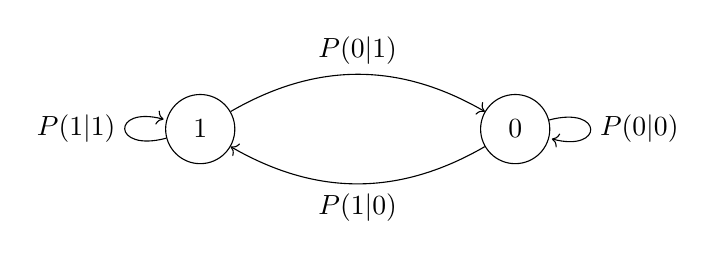
\begin{tikzpicture}[node distance = 4cm]

\node[state] (present) {$1$};
\node[state, right of=present] (absent) {$0$};

\path[->] (present) 	edge [bend left]		
							node [above] {$P(0|1)$} (absent)
						(absent) 	edge [bend left]		
							node [below] {$P(1|0)$} (present)
						(present) 	edge [loop left]		
							node [left] {$P(1|1)$} (present)
						(absent) 	edge [loop right]		
							node [right] {$P(0|0)$} (absent);
\end{tikzpicture}
\end{center}
\caption{
	\label{dia:simple_mc}
	Representació del patró de la cadena de Markov de grau 1 i homogènia en temps discret a emprar per a modelar l'evolució de la presència de cada un dels usuaris al CV de la UOC. 
}
\end{figure}

Molt sovint es sintetitza el seu comportament en una matriu de transicions

$$
\begin{pmatrix}
P(0|0) & P(1|0) \\
P(0|1) & P(1|1)
\end{pmatrix}
$$

en què les files corresponen als possibles valors de $a_j$ i les columnes als de $a_{j+1}$. Ara bé, per la regla de la suma, en un espai d'estats binari com el nostre, l'obtenció de la matriu de transicions es redueix a l'estimació de dos paràmetres $\alpha$ i $\beta$ de la manera següent:

$$
\begin{pmatrix}
1 - \alpha & \alpha \\
1 - \beta & \beta
\end{pmatrix}
$$

\subsection{Estimació de models}

Noti's que els valors concrets que puguin prendre el parell de paràmetres $\alpha$ i $\beta$ es poden interpretar com una caracterització del comportament d'un usuari pel que fa la seva presència al CV de la UOC. És a dir, podem reduir les tuples que pertanyen, respectivament, a \mt{user\_days} i \mt{user\_weeks} als atributs \mt{user\_id}, $\mt{alpha} = \alpha$ i $\mt{beta} = \beta$. Per a cada usuari $i$-èssim, mirarem d'estimar quins són els valors de $\alpha$ i $\beta$ que defineixen la DTMC de grau 1 homogènia que és més probable que hagi generat la seqüència de valors booleans presents en $a_{i,0},\ldots,a_{i,m}$ que li corresponen. 

En primer lloc, val a dir que, per què l'estimació tingui sentit, cal prescindir d'aquells usuaris que presentin el valor 1 per tot $a_j$ ($j \in [0,m]$)\footnote{Noti's que, per la naturalesa mateixa de les dades sobre què estem treballant, és impossible que hi hagi cap usuari que presenti el valor 0 per a tot $a_j$}, el nombre dels quals ha resultat ser menyspreable (en el cas de \mt{user\_days} no n'hi ha hagut cap, i solament 2 en \mt{user\_weeks}). Fet això, per a estimar $\alpha$ i $\beta$ s'ha emprat el mètode de la màxima versemblança (MLE). En general, si $S$ és el conjunt d'estats possibles i  $x,y,z \in S$, s'estima $P(y|x)$ tot calculant el paràmetre $\widehat{p}_{x,y}$ de la manera següent \citep{spedicato14}\footnote{Així és com es realitza l'estimació en la funció \mt{markovchainFit} del paquet \mt{markovchain} de R que he emprat.}:

$$
	\widehat{p}_{x,y} = \frac{n_{x,y}}{ \displaystyle \sum_{z \in \{0,1\}} n_{x,z}} 
$$   

On $n_{x,y}$ indica el nombre transicions de $x$ a $y$ que s'han observat. Per tant, $\alpha$ i $\beta$ s'han obtingut de la manera següent:

\begin{align*}
\alpha & = \frac{n_{0,1}}{ \displaystyle \sum_{z \in \{0,1\}} n_{0,z}} &
\beta & = \frac{n_{1,1}}{ \displaystyle \sum_{z \in \{0,1\}} n_{1,z}}
\end{align*}

\subsection{Dispersió dels resultats}

Passem tot seguit a mostrar els resultats de l'estimació de $\alpha$ i $\beta$ per a cada element de \mt{user\_days} i \mt{user\_weeks}. A la gràfica de la figura \ref{graph:mc_params_days} es mostra un diagrama de dispersió on es situa cada cas de \mt{user\_days} en funció dels valors de $\alpha$ i $\beta$. A la de la figura \ref{graph:mc_params_weeks} es fa el mateix per als elements de \mt{user\_weeks}. Observi's que en tots dos casos, tal com s'havia fet en el diagrama de la figura \ref{graph:user_first_last_scatter}, els punts presenten certa transparència (el canal \emph{alpha} és reduït al 10\%) per poder apreciar-ne millor les aglomeracions.  

\begin{figure}
\begin{center}
\includegraphics[width=10cm]{mc_params_days}
\caption{
\label{graph:mc_params_days}
	Diagrama de dispersió on es representen els valors de $\alpha$ i $\beta$ per als elements de \mt{user\_days}.
}
\end{center}
\end{figure}

Si bé la finalitat d'emprar el model de les cadenes de Markov era mirar de reflectir millor la naturalesa estocàstica de l'evolució de la presència de cada usuari al CV de la UOC. A més, la simple estimació de $\alpha$ i $\beta$ era especialment atractiva ja que permet reduir-ne la caracterització a dos camps i evitar els inconvenients d'emprar els $m+1$ atributs (recodem que $m = 119$ per a \mt{user\_days} i $m = 17$ per a \mt{user\_weeks}), com ja es pot copsar a primer cop d'ull, \emph{els resultats no són especialment esperançadors}.  

En el diagrama de la figura \ref{graph:mc_params_days} els casos estan repartits d'una manera tan uniforme en el pla que es fa virtualment inviable el reconeixement de \emph{clusters} de tal manera que aquests ens proporcionin una informació útil. I és que si bé és possible aplicar mètodes de \emph{clustering} en una mostra com aquesta, com és obvi, les agregacions obtingudes ens seran de poca utilitat, ja que l'homogeneïtat de la distribució dels casos els resta poder explicatiu. Pel que fa els resultats sobre \mt{user\_weeks}, que es mostren a la figura \ref{graph:mc_params_days}, presenten algunes diferències, tot i que aconsegueixen esquivar les mateixes dificultats. En aquest cas, gran quantitat d'usuaris es superposen d'una manera quasi exacta en certs punts concrets del pla. Això és una conseqüència natural del fet que les cadenes de valors booleans a partir de les quals hem estimat els paràmetres presentin una longitud menor, ja que aquest fenomen redueix l'espai de possibles valors de $n_{x,y}$. Malgrat tot, la distribució dels casos en el pla és, en general, igualment homogènia, i un procés de reconeixement de \emph{clusters} donaria lloc a resultats igualment infructuosos.            
 
\begin{figure}
\begin{center}
\includegraphics[width=10cm]{mc_params_weeks}
\caption{
\label{graph:mc_params_weeks}
	Diagrama de dispersió on es representen els valors de $\alpha$ i $\beta$ per als elements de \mt{user\_weeks}. 
}
\end{center}
\end{figure}

Evidentment, poden ésser moltes i molt variades les raons de la inviabilitat d'aquest model, ja que, al cap hi a la fi, ja hem reconegut d'entrada la simplificació que comporta. Potser caldria augmentar el grau de la cadena de Markov, o bé no fer-la homogènia en el temps i fer variar les probabilitats de les transicions en funció del moment del temps representat. Tot i això, he decidit no seguir en aquesta direcció, ja que em sembla haver trobat un model molt millor, que mantingui la simplicitat i, a la vegada, ofereixi prediccions útils per als nostres propòsits.  

\section{Modelat mitjançant models ocults de Markov}

Si bé tot model és una simplificació, el que hem triat en la secció anterior  pateix d'un enfocament massa ingenu. En ell estàvem fent dependre la presència o absència d'un alumne al CV en un interval $I_j$ només de la presència o absència del mateix alumne en l'interval $I_{j-1}$. Com és natural, hem obtingut un perfil diferent per a cada combinació possible de valors de $a_j$, perfil que, a més, només hem pogut produir \emph{a posteriori}. 

Tanmateix, com apuntava en la secció \ref{sec:clustering_utility}, no és pas aquesta informació la que ens interessa, sinó més aviat la probabilitat que un usuari qualsevol hagi abandonat el curs per a cada interval $I_j$. És a dir, per a cada seqüència de valors $a_{i,0}, \ldots, a_{i,k}$, corresponents a l'usuari $i$-èssim, ens interessa saber quina és la probabilitat que per tot $a_{i,j} = 0$ amb $k < j \leq m$. A més, seria òptim poder obtenir aquesta informació \emph{a priori}, és a dir, \emph{mentre} ens trobem en el transcurs de l'interval $I_k$ o en un moment anterior. D'aquesta manera sí que podríem predir l'abandó per part d'usuaris del campus (una part dels quals sabem que són estudiants matriculats) abans que hagi finalitzat el semestre.

Com es veurà tot seguit, pretenc haver aconseguit un model que satisfà totes aquestes condicions i que, a més, manté una simplicitat notable. El model en qüestió és un cas concret del model ocult de Markov (HMM). 

\subsection{Descripció del model}

Com és ben sabut \citep[p. 588-91,835]{russell09}, en un HMM els diferents estats concrets, és a dir, els valors  que prenen cada una de les variables $x_j$ que componen la seqüència estocàstica es suposen desconeguts. Tot i això, per a cada variable oculta $x_j$ se n'afegeix una de nova $y_j$ el valor que prengui (és a dir, l'estat en què es trobi) sí que serà conegut i dependrà de la probabilitat condicional $P(y_j|x_j)$. En la figura \ref{dia:hmm_evo} es mostra una representació gràfica de l'evolució temporal d'aquest sistema.            

\begin{figure}
\begin{center}
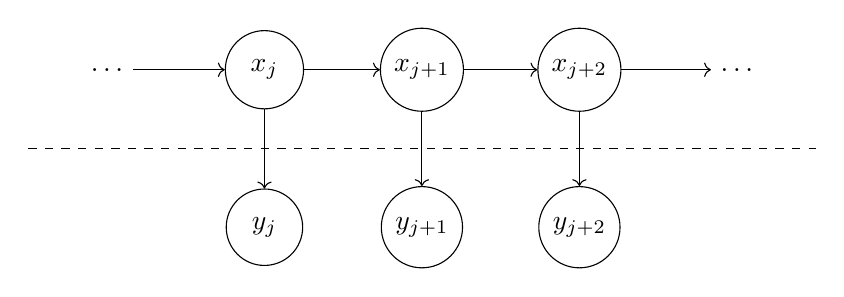
\begin{tikzpicture}[node distance = 2cm]

\node[inner sep = 2mm, state] (q_0) {$x_j$};
\node[left of=q_0] (ldots) {$\ldots$};
\node[state, right of=q_0] (q_1) {$x_{j+1}$};
\node[state, right of=q_1] (q_2) {$x_{j+2}$};
\node[right of=q_2] (rdots) {$\ldots$};

\node[inner sep = 2mm, state, below of=q_0] (e_0) {$y_j$};
\node[state, below of=q_1] (e_1) {$y_{j+1}$};
\node[state, below of=q_2] (e_2) {$y_{j+2}$};

\draw[->] (ldots) -- (q_0);
\draw[->] (q_0) -- (q_1);
\draw[->] (q_1) -- (q_2);
\draw[->] (q_2) -- (rdots);

\draw[->] (q_0) -- (e_0);
\draw[->] (q_1) -- (e_1);
\draw[->] (q_2) -- (e_2);							
\draw[dashed] (-3,-1) -- (7,-1);						
							
\end{tikzpicture}
\end{center}
\caption{
	\label{dia:hmm_evo}
	Esquema de l'evolució temporal d'un model ocult de Markov.
}
\end{figure}

Així doncs, en aquest cas l'estructura del HMM vindrà definida per:

\begin{enumerate}[(1)]
	\item Un espai d'estats $S$ que poden prendre les variables $x_j$ que conformen la cadena de Markov oculta.
	\item Un espai d'estats $E$ (noti's que és possible que $S \neq E$) que poden prendre les variables observables $y_i$. 
	\item Un estat inicial $s_0 \in S$.  
	\item Una matriu de transicions dels estats de la cadena de Markov oculta.
	\item Una matriu d'emissions que expressi la probabilitat $P(y|x)$ d'observar cada emissió $y$ condicionada per la probabilitat de l'estat $x$.   
\end{enumerate}

Tot tenint present aquest esquema general, podem modelar el cas que ens ocupa de la manera següent:

\begin{enumerate}[(1)]

\item Suposarem que cada usuari pot trobar-se, per a cada interval $I_j$, en un dels dos estats del conjunt $S = \{A,Q\}$ en funció del següent:

	\begin{enumerate}[i.]
	\item L'usuari pot ésser \emph{actiu}, és a dir, que \emph{està pendent} d'allò que s'esdevé al CV. Anomenarem $A$ aquest estat.
	\item Per contra, també pot \emph{haver abandonat} el CV, això és, que no tornarà a establir-hi cap sessió fins a final de semestre. Anomenarem $Q$ aquest segon estat.   
	\end{enumerate}

\item Considerarem que tots els usuaris comencen el semestre essent actius, és a dir, que no n'hi ha cap que, durant el primer interval $I_0$ ja hagi abandonat. Per tant l'estat inicial serà $A$. 
	
\item Per altra banda, considerarem ara els valors de $a_{i,0},\ldots,s_{i,m}$ com les emissions per part de les variables ocultes corresponents del model a què pertany a l'usuari $i$-èssim. Així doncs, l'espai d'estats variables observables és $E = \{0,1\}$

\item Per definició, si un usuari ha abandonat el CV ja no tornarà a connectar-s'hi. Per tant, considerarem que $Q$ és un estat absorvent, és a dir, que $P(A|Q) = 0$ i $P(Q|Q) = 1$. D'aquesta manera, la matriu de transicions tindrà l'aspecte següent:

$$
\begin{pmatrix}
P(Q|Q) & P(A|Q) \\
P(Q|A) & P(A|A)
\end{pmatrix}
=
\begin{pmatrix}
1 & 0 \\
1- \alpha & \alpha
\end{pmatrix}
$$

On $\alpha$ és un dels paràmetres que determina el model a estimar.

\item Per altra banda, també és obvi que si un usuari ha trencat la reva relació amb el CV, aleshores tampoc ja no hi establirà més sessions. És a dir, $P(0|Q) = 1$ i $P(1|Q) = 0$. Consegüentment, la matriu d'emissions és:

$$
\begin{pmatrix}
P(0|Q) & P(1|Q) \\
P(0|A) & P(1|A)
\end{pmatrix}
=
\begin{pmatrix}
1 & 0 \\
1 - \beta & \beta
\end{pmatrix}
$$

On $\beta$ és l'altre dels paràmetres a estimar. 
\end{enumerate} 

En la figura \ref{dia:simple_hmm} pot veure's un esquema gràfic del model que acabem de descriure.

\begin{figure}
\begin{center}
\begin{tikzpicture}[node distance = 4cm]

\node[state, above of=present] (active) {$A$};
\node[state, above of=absent] (quit) {$Q$}; 

\node[state] (present) {$1$};
\node[state, right of=present] (absent) {$0$};

\path[->] (active) 	edge [bend left]		
							node [above] {$1 - \alpha$} (quit)
						(quit) 	edge [bend left]		
							node [below] {$0$} (active)
						(active) 	edge [loop left]		
							node [left] {$\alpha$} (active)
						(quit) 	edge [loop right]		
							node [right] {$1$} (quit);
							
\path[->] (active) edge [bend right] 
							node [left] {$\beta$} (present)
						(active) edge [bend right] 
							node [below left] {$1 -\beta$} (absent)
						(quit) edge [bend left]
							node [below right] {$0$} (present)
						(quit) edge [bend left]
							node [right] {$1$} (absent);	
							
\draw[dashed] (-3,2.75) -- (7,2.75);						
							
\end{tikzpicture}
\end{center}
\caption{
	\label{dia:simple_hmm}
	Esquema del model ocult de Markov per a predir l'abandonament, per part dels usuaris, de la relació amb el CV. 
}
\end{figure}

Així doncs, hem reduït la solució del problema a la tasca d'haver d'estimar els dos paràmetres $\alpha$ i $\beta$. 

\subsection{Estimació de paràmetres}

Com durem a terme aquesta estimació? En vistes a una validació creuada, ho farem a partir d'una mostra que anomenarem \mt{users\_train}, independement de si és un subconjunt de \mt{user\_days} o de \mt{user\_weeks}. Per altra banda, si bé és cert que hi ha una gran varietat d'algoritmes per a estimar els paràmetres d'un HMM n'hi haurà prou emprant un mètode molt simple. 

Notem en primer lloc, que $\alpha$ és la probabilitat que un usuari que es troba actiu durant un interval $I_j$, segueixi essent-ho durant l'immediatament posterior $I_{j+1}$. Per definició, sabem que com a mínim per a un 50\% dels usuaris, aquests es trobaran actius des de l'interval $I_0$ fins aquell que inclou la mediana mostral $q_{50\%}(\mt{l\_sess})$ dels valors que pren en el conjunt d'entrenament \mt{users\_train} el camp \mt{l\_sess}, el qual indica, recordem, quin és el \mt{central\_activity\_point} de la darrera sessió de l'usuari. Podem aproximar aquest fet tot suposant que, si prenem un usuari qualsevol, la probabilitat que aquest encara sigui actiu en l'interval $I_j$ que conté el valor d'aquesta mediana, és de 0.5.   

Per altra banda recordem que, en una DTMC, si coneixem la distribució de probabilitats de l'estat inicial podem preveure la probabilitat de l'estat en el pas $j$-èssim. Per al nostre model concret, si definim $\lambda \in [0,m]$ com l'índex de l'interval que conté ${q_{50\%}(\mt{l\_sess})}$ l'operació que proporciona aquesta informació és la següent:    

\begin{align*}
\begin{pmatrix}
P(Q) & P(A)
\end{pmatrix}
\begin{pmatrix}
P(Q|Q) & P(A|Q) \\
P(Q|A) & P(A|A)
\end{pmatrix}^\lambda
 = & 
\begin{pmatrix}
0 & 1
\end{pmatrix}
\begin{pmatrix}
1 & 0 \\
1 - \alpha & \alpha
\end{pmatrix}^\lambda
\\
= &
\begin{pmatrix}
1-\alpha^\lambda & \alpha^\lambda
\end{pmatrix}
\end{align*}   

Sabem, doncs, que $\alpha^{\lambda}$ és la probabilitat de $P(A)$ en l'interval $I_{\lambda}$. Però ja hem dit que aproximaríem aquest valor a $0.5$. Per tant:

$$
 \alpha^{\lambda} = \frac{1}{2} \Rightarrow \alpha = \left(\frac{1}{2}\right)^{\frac{1}{\lambda}} 	
$$

Hem pres una mostra aleatòria del 50\% per a confeccionar \mt{train\_users} en cada cas i, n'hem obtingut els valors següents:

\begin{enumerate}
	\item Per a \mt{train\_users} $\subseteq$ \mt{user\_days}
		$$
			\lambda = 113 \Rightarrow \alpha = 0.9938847
		$$ 
	\item Per a \mt{train\_users} $\subseteq$ \mt{user\_weeks}	
		$$
			\lambda = 16 \Rightarrow \alpha = 0.9576033
		$$
\end{enumerate}

Mirem ara d'estimar $\beta$. Noti's que aquest paràmetre representa la probabilitat que un usuari estableixi alguna sessió durant un iterval qualsevol mentre es troba actiu (estat $A$). Així, doncs, per a cada $\mt{user}_i$ podem definir la subseqüència de valors booleans $a_{i,0},\ldots,a_{i,u}$ ($u \leq m$) tal que $\mt{user}_i.\mt{l\_sess} \in I_u$, és a dir, la subseqüència durant la qual ha mantingut aquest estat. Així, definirem el nou camp següent per a cada usuari $i$-èssim, 

$$
	\mt{user}_i.\mt{a\_rate} = \frac{1}{u+1} \sum_{j = 0}^u a_{i,j}
$$ 

que representa la \emph{taxa de presència} al CV de la UOC que aquest usuari ha tingut mentre encara no l'ha abandonat. 

El paràmetre $\beta$ l'estimarem simplement prenent la mitjana mostral del valor d'aquest nou camp:

$$
	\beta = \overline{\mt{a\_rate}} = \frac{1}{|\mt{train\_users}|} \sum_{v \in \mt{train\_users}} v.\mt{a\_rate}
$$

Els valors concrets obtinguts són:

\begin{enumerate}
	\item Per a \mt{train\_users} $\subseteq$ \mt{user\_days}
		$$
			 \beta = 0.4087153
		$$ 
	\item Per a \mt{train\_users} $\subseteq$ \mt{user\_weeks}	
		$$
			 \beta = 0.7235815
		$$
\end{enumerate}

\subsection{Resultats de la predicció}

Ja estem en condicions, doncs, de validar el nostre model. El conjunt de validació pres ha estat, simplement en complementari 
$$
\mt{users\_test} = \mt{users\_train}^C
$$
en \mt{user\_days} i \mt{user\_weeks}, respectivament. 

Obervi's que en realitat es fa una predicció per a cada interval de la discretització en funció de $d$. És a dir, per a cada interval $I_j$, el model predirà quin és l'estat ocult en el qual és més probable que es trobi l'usuari $i$-èssim en funció de la seqüència d'observacions $a_{i,0},\ldots,a_{0,j-1}$ i dels paràmetres que acabem d'estimar. La predicció en qüestió l'he realitzada per mitjà de l'aplicació de l'\emph{algoritme de Viterbi} \citep{viterbi67} \footnote{Aquest és l'algoritme que segueix la funció \mt{viterbi} inclosa en el paquet d'R que porta per nom \mt{HMM} \citep{himmelmann10}.}. 

Per a cada interval $I_j$ amb $j \in [1,m]$, doncs, podem construir una matriu de confusió com la que es mostra a continuació, els valors de la qual avaluen la utilitat del model a l'hora de predir si l'usuari ja ha abandonat el CV en aquest interval. 

$$
\begin{pmatrix}
TP & FP \\
TN & FN
\end{pmatrix}_j
$$

Noti's que les files es refereixen, en l'ordre $\langle Q, A \rangle$, als valors observats que corresponen als estats de la cadena oculta de Markov, i les columnes, també en el mateix ordre, als valors observats. Les inicials dels valors indicats signifiquen, per tant:

\begin{enumerate}[(1)]
\item $TP$ (\emph{True Positives}): El nombre d'usuaris en què s'ha predit que es trobaven en l'estat $Q$ i la predicció ha estat correcta.  
\item $TN$ (\emph{True Negatives}): El nombre d'usuaris en què s'ha predit que es trobaven en l'estat $A$ i la predicció ha estat correcta.
\item $FP$ (\emph{False Positives}): El nombre d'usuaris en què s'ha predit que es trobaven en l'estat $Q$ i la predicció ha estat incorrecta. 
\item $FN$ (\emph{False Negatives}): El nombre d'usuaris en què s'ha predit que es trobaven en l'estat $A$ i la predicció ha estat incorrecta.
\end{enumerate}

En les figures \ref{graph:hmm_days_confusion_m_day} i \ref{graph:hmm_weeks_confusion_m_day} s'hi mostren, en percentatges, les evolucions respectives d'alguns d'aquests valors en funció del temps per a \mt{user\_days} i \mt{user\_weeks}. 

\begin{figure*}
\begin{center}
\includegraphics{hmm_days_confusion_m_day}
\caption{
\label{graph:hmm_days_confusion_m_day}
	Evolució dels valors de la matriu de confusió en funció del temps per a \mt{user\_days}	
}
\end{center}
\end{figure*}

Les variables que hi apareixen es calculen com s'indica tot seguit:

\begin{align*}
\mt{accuracy} = & 100 \frac{TP + TN}{TP + TN + FP + FN} & 
\mt{false\_negatives} = & 100 \frac{FN}{TP + TN + FP + FN} \\
\mt{false\_positives} = & 100 \frac{FN}{TP + TN + FP + FN} & 
\mt{quit\_users} = & 100 \frac{TP + FN}{TP + TN + FP + FN} 
\end{align*}

Observi's que en el primer cas la precisió del model és força pobra a partir de finals de setembre però millora a mesura que avança el semestres. Per altra banda, cosa que és més rellevant, la major part de les errades consisteixen en falsos positius, és a dir, prediccions d'abandonament per part d'usuaris que en realitat seguien actius. Això és un mal menor ja que el que ens importa, en vistes a la millora del procés educatiu, és evitar que ens passin per alt abandonaments, és a dir, els falsos negatius.  

\begin{figure*}
\begin{center}
\includegraphics{hmm_weeks_confusion_m_day}
\caption{
\label{graph:hmm_weeks_confusion_m_day}
	Evolució dels valors de la matriu de confusió en funció del temps per a \mt{user\_weeks}	
}
\end{center}
\end{figure*}

Per acabar, notem que la fiabilitat del model en la discretització per setmanes és molt més alta. La precisió és del 100\% des de l'inici del semestre fins a final d'any.

\chapter{Conclusions}

Clourem aquest treball tot fent una síntesi dels resultats més valuosos que hem pogut recollir de l'estudi que presenta. 

\section{Utilitat de la discretització}

Recordem en primer lloc que les dades que hem rebut presenten, en resum, les dificultats següents:

\begin{enumerate}[(1)]

\item No coneixem en cap mesura el procés que ha donat lloc a llur generació. Per tant, no sabem fins a quin punt el detall dels valors dels camps que inclouen són un bon reflex dels fets que representen.

\item Tampoc sabem si cada un dels usuaris representats per part dels identificators que apareixen en les dades corresponen o no a estudiants de la UOC, que són l'objecte que ens interessa en aquest estudi.

\item En darrer terme, fins i tot si un identificador d'usuari pertany a un estudiant, també és ben poca la informació que cada element de \mt{sessions} proporciona sobre el procés d'aprenentatge en què es troba immers.   
  
\end{enumerate} 

Així, doncs, la mètrica presència / absència per interval de temps per a cada usuari és una manera d'extraure informació fiable a partir de les dades en brut. De fet, a partir d'elles, és ben poc el que es pot dels usuaris més enllà del que expressa aquesta variable. 

\section{Agregació per $k$-\emph{means} per a identificar tipus de comportament}

L'aplicació del mètode $k$-\emph{means} a partir del resultat de la discretització ha estat reeïxida a l'hora d'identificar una jerarquia de perfils de comportament dels usuaris pel que fa llur relació amb el CV durant el transcurs del semestre. Tot i que no sapiguem quins usuaris són estudiants, noti's que aquesta tipologia és útil per als propòsits de la \emph{EDM\&LA} ja que, no només inclouen la caracterització dels que sí que ho són, sinó que estableixen un primer criteri per a discriminar-los respecte altres.   

\section{L'eficàcia predictiva dels models ocults de Markov}  

En darrer lloc, entenc que el resultat més valuós de l'estudi que s'exposa en aquesta memòria és el model ocult de Markov (HMM) els paràmetres dels quals són determinats d'una manera especialment simple. Pel que fa la seva precisió a l'hora de predir els abandonaments per part dels usuaris ha estat del 100\% fins a finals de desembre pel cas de la discretització setmanal. 

A més, aquesta predicció segueix essent útil pel que fa els nostres objectius encara que no poguem saber quins dels usuaris són estudiants, ja que l'avís d'abandó és igualment eficaç per a tots ells, i és d'esperar que una aplicació pràctica d'aquest model ja faci aquesta distinció.  	  
 
\backmatter

\bibliography{aadroher_uoc_tfg}




\end{document}

